\documentclass[14pt,a4paper,UTF8,twoside]{article}

% Formatting Packages ——————————————————————————————————————
\usepackage{multicol} % 多行多列包
\usepackage{multirow}
\usepackage{enumitem} % 数字编号包
\usepackage{indentfirst}
\usepackage[toc]{multitoc} % 多行目录包

% Math & Physics Packages ————————————————————————————
\usepackage{amsmath, amsthm, amsfonts, amssymb} % 基础数学包
\usepackage{setspace}
\usepackage{physics}
\usepackage{cancel}
\usepackage{nicefrac}
\usepackage{unicode-math} % 允许数学公式使用特定字体
\usepackage{mdframed} % 注释包

% Image-related Packages —————————————————————————————
\usepackage{graphicx} % 插入图片要这个包
\usepackage{float} % 浮动体环境,用来调整图片的位置
\usepackage{subcaption} % 子图包
\usepackage{pgfgantt}
\usepackage{graphics, graphicx}
\usepackage{tikz, tikz-qtree}
\usetikzlibrary{arrows.meta, positioning, shapes}
\usetikzlibrary{shapes.geometric}
\tikzstyle{node_style} = [rectangle, rounded corners, draw, align=center, text width=3cm, minimum height=0.65cm]
\tikzstyle{arrow_style} = [thick, ->, >=stealth]

\usepackage{pgfplots}
\pgfplotsset{compat=1.18}
\usepackage{xcolor}
\usepackage{fourier-orns}
\usepackage{lipsum}

% 其余常用包 ————————————————————————————————————————————
\usepackage{booktabs} % 表格库
\usepackage{titlesec} % 标题库
\usepackage{fancyhdr} % 页眉页脚库
\usepackage[sorting=none]{biblatex}
\usepackage{array}

%—————————————页面基础设置———————————————%

\usepackage{geometry}
\geometry{left=10mm, right=10mm, top=20mm, bottom=20mm}
% 这个命令用来设置纸张上下左右的间距,可以自己调调试试

% 字体设置 ————————————————————————————————————————————————
\usepackage{fontspec} % 允许设置字体
\usepackage[utf8]{inputenc}
\usepackage{ctex}

% 代码块包 ————————————————————————————————————————————————
\usepackage{listings}

% ————————————————————————————————————————————————————————

% 导言区
% Colour Palette ——————————————————————————————————————
\definecolor{merah}{HTML}{F4564E}
\definecolor{merahtua}{HTML}{89313E}
\definecolor{biru}{HTML}{60BBE5}
\definecolor{birutua}{HTML}{412F66}
\definecolor{hijau}{HTML}{59CC78}
\definecolor{hijautua}{HTML}{366D5B}
\definecolor{kuning}{HTML}{FFD56B}
\definecolor{jingga}{HTML}{FBA15F}
\definecolor{ungu}{HTML}{8C5FBF}
\definecolor{lavender}{HTML}{CBA5E8}
\definecolor{merjamb}{HTML}{FFB6E0}
\definecolor{mygray}{HTML}{E6E6E6}
\definecolor{mygreen}{rgb}{0,0.6,0}
\definecolor{mymauve}{rgb}{0.58,0,0.82}

\lstset {
    backgroundcolor=\color{white},   % choose the background color; you must add \usepackage{color} or \usepackage{xcolor}
    basicstyle=\small\ttfamily,        % the size of the fonts that are used for the code
    breakatwhitespace=false,         % sets if automatic breaks should only happen at whitespace
    breaklines=true,                 % sets automatic line breaking
    captionpos=bl,                   % sets the caption-position to bottom
    commentstyle=\color{mygreen},    % comment style
    deletekeywords={...},            % if you want to delete keywords from the given language
    escapeinside={\%*}{*},           % if you want to add LaTeX within your code
    extendedchars=true,              % lets you use non-ASCII characters; for 8-bits encodings only, does not work with UTF-8
    frame=single,                    % adds a frame around the code
    keepspaces=true,                 % keeps spaces in text, useful for keeping indentation of code (possibly needs columns=flexible)
    keywordstyle=\color{blue},       % keyword style
    % language=Python,               % the language of the code
    morekeywords={*,...},            % if you want to add more keywords to the set
    numbers=left,                    % where to put the line-numbers; possible values are (none, left, right)
    numbersep=5pt,                   % how far the line-numbers are from the code
    numberstyle=\tiny\color{mygray}, % the style that is used for the line-numbers
    rulecolor=\color{black},         % if not set, the frame-color may be changed on line-breaks within not-black text (e.g. comments (green here))
    showspaces=false,                % show spaces everywhere adding particular underscores; it overrides 'showstringspaces'
    showstringspaces=false,          % underline spaces within strings only
    showtabs=false,                  % show tabs within strings adding particular underscores
    stepnumber=1,                    % the step between two line-numbers. If it's 1, each line will be numbered
    stringstyle=\color{orange},      % string literal style
    tabsize=2,                       % sets default tabsize to 2 spaces
    % title=Python Code              % show the filename of files included with \lstinputlisting; also try caption instead of title
}

\author{10233903433 胡盛扉}
\title{\huge{中国省级年度夜间灯光强度交互式地图} \\ \Large{——软件工程与GIS开发课程作业 \hspace{0.1em} 说明文档}}

\begin{document}
\maketitle

\section{介绍}
本项目旨在开发一个交互式的Web应用程序,用于可视化和分析中国各省级市级行政区的年度夜间灯光强度数据。该系统利用Streamlit框架构建用户界面,结合Folium库和Pydeck库生成地理空间数据地图,并使用Plotly Express库展示时间序列趋势。用户可以通过该系统直观地观察不同年份、不同省份的夜间灯光强度分布,并探索其随时间的变化趋势。同时,在其他选项中勾选“查看市级灯光强度标记簇”,也可以查看中国各个市级的夜间灯光数据。夜间灯光数据是衡量区域经济活动、城市化进程和能源消耗等的重要指标,用户可以在这个应用程序中深入了解中国各地区的夜间灯光强度变化。

值得一提的是,本应用的夜间灯光值指的是平均值,其计算方法是将每个省份的所有像元值总和除以该省份所占的像元数,市级的夜间灯光值同理。
\section{主要功能}
本项目主要包含以下核心功能:
\begin{itemize}
    \item \textbf{交互式夜间灯光地图}:
    \begin{figure}[H]
        \centering
        \fbox{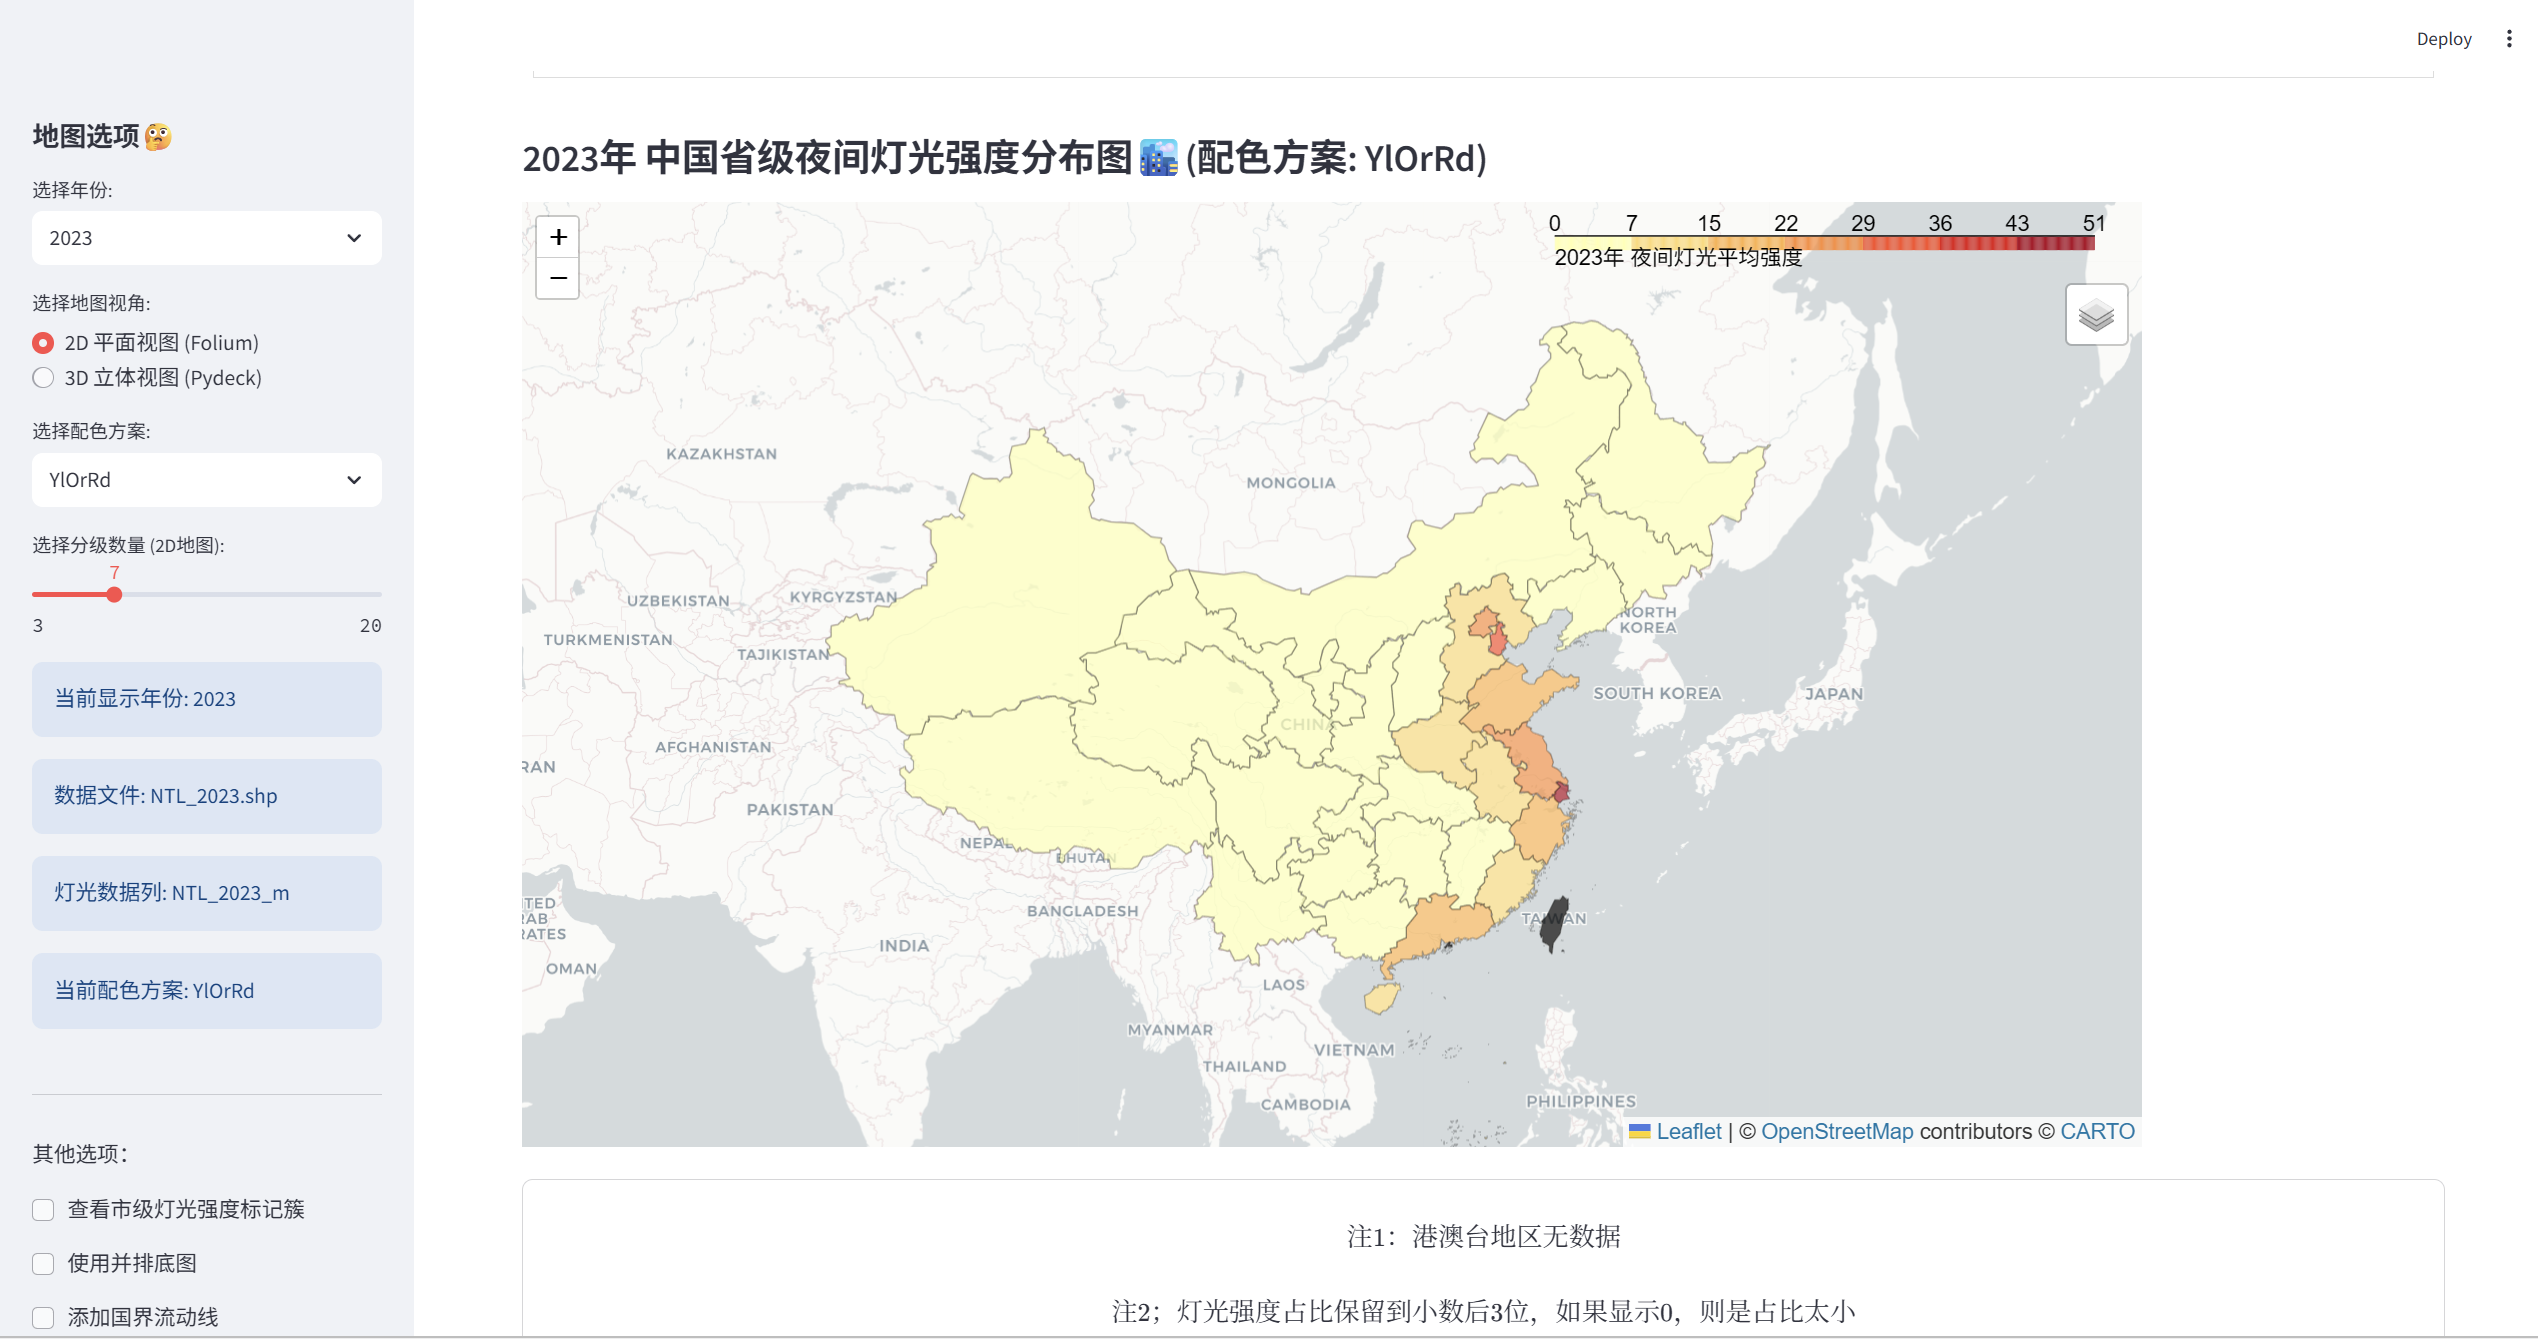
\includegraphics[width=0.8\textwidth]{fig/overall_map_true.png}}
        \caption{交互式夜间灯光地图概览}
        \label{fig:interactive_map_example}
    \end{figure}
    \begin{itemize}
        \item 用户可以在侧边栏选择特定年份来查看该年份的省级夜间灯光数据,地图也以分层设色的方式展示各省的灯光强度。
        \item 用户可以自定义地图的配色方案,添加并排底图以及国界流动线以适应不同的可视化需求。
        \item 用户还可以在侧边栏选择查看市级灯光强度标记簇,这样可以在地图上显示各市级的夜间灯光强度数据,为更精细的分析提供支持。
        \item 鼠标悬停在地图上的省份区域时,会显示该省份的名称及当年的夜间灯光强度值。
        \item 因为程序计算量略大,加载时间长,我因此嵌入了一个HTML小游戏,通过点击按钮,可以减少等待时间的无聊感。
        \begin{figure}[H]
            \centering
            \fbox{
\includegraphics[width=0.8\textwidth]{fig/html_game.png}}
            \caption{小游戏示例}
            \label{fig:game_example}
        \end{figure}
    \end{itemize}
    \item \textbf{夜间灯光强度历年变化趋势动画}:
    \begin{itemize}
        \item 用户可以播放动画折线图,这个图展示所有省份从起始年份到选定年份的夜间灯光强度累积变化过程,用户可以通过动画播放控件观察各省份灯光强度随时间演变的动态。
        \item 对图例进行单击操作可以隐藏特定省份,双击可以只呈现特定省份,提高了图表的可读性和交互性。
    \end{itemize}
    \begin{figure}[H]
    \centering
    \begin{minipage}{.45\linewidth}
    \centering
    \fbox{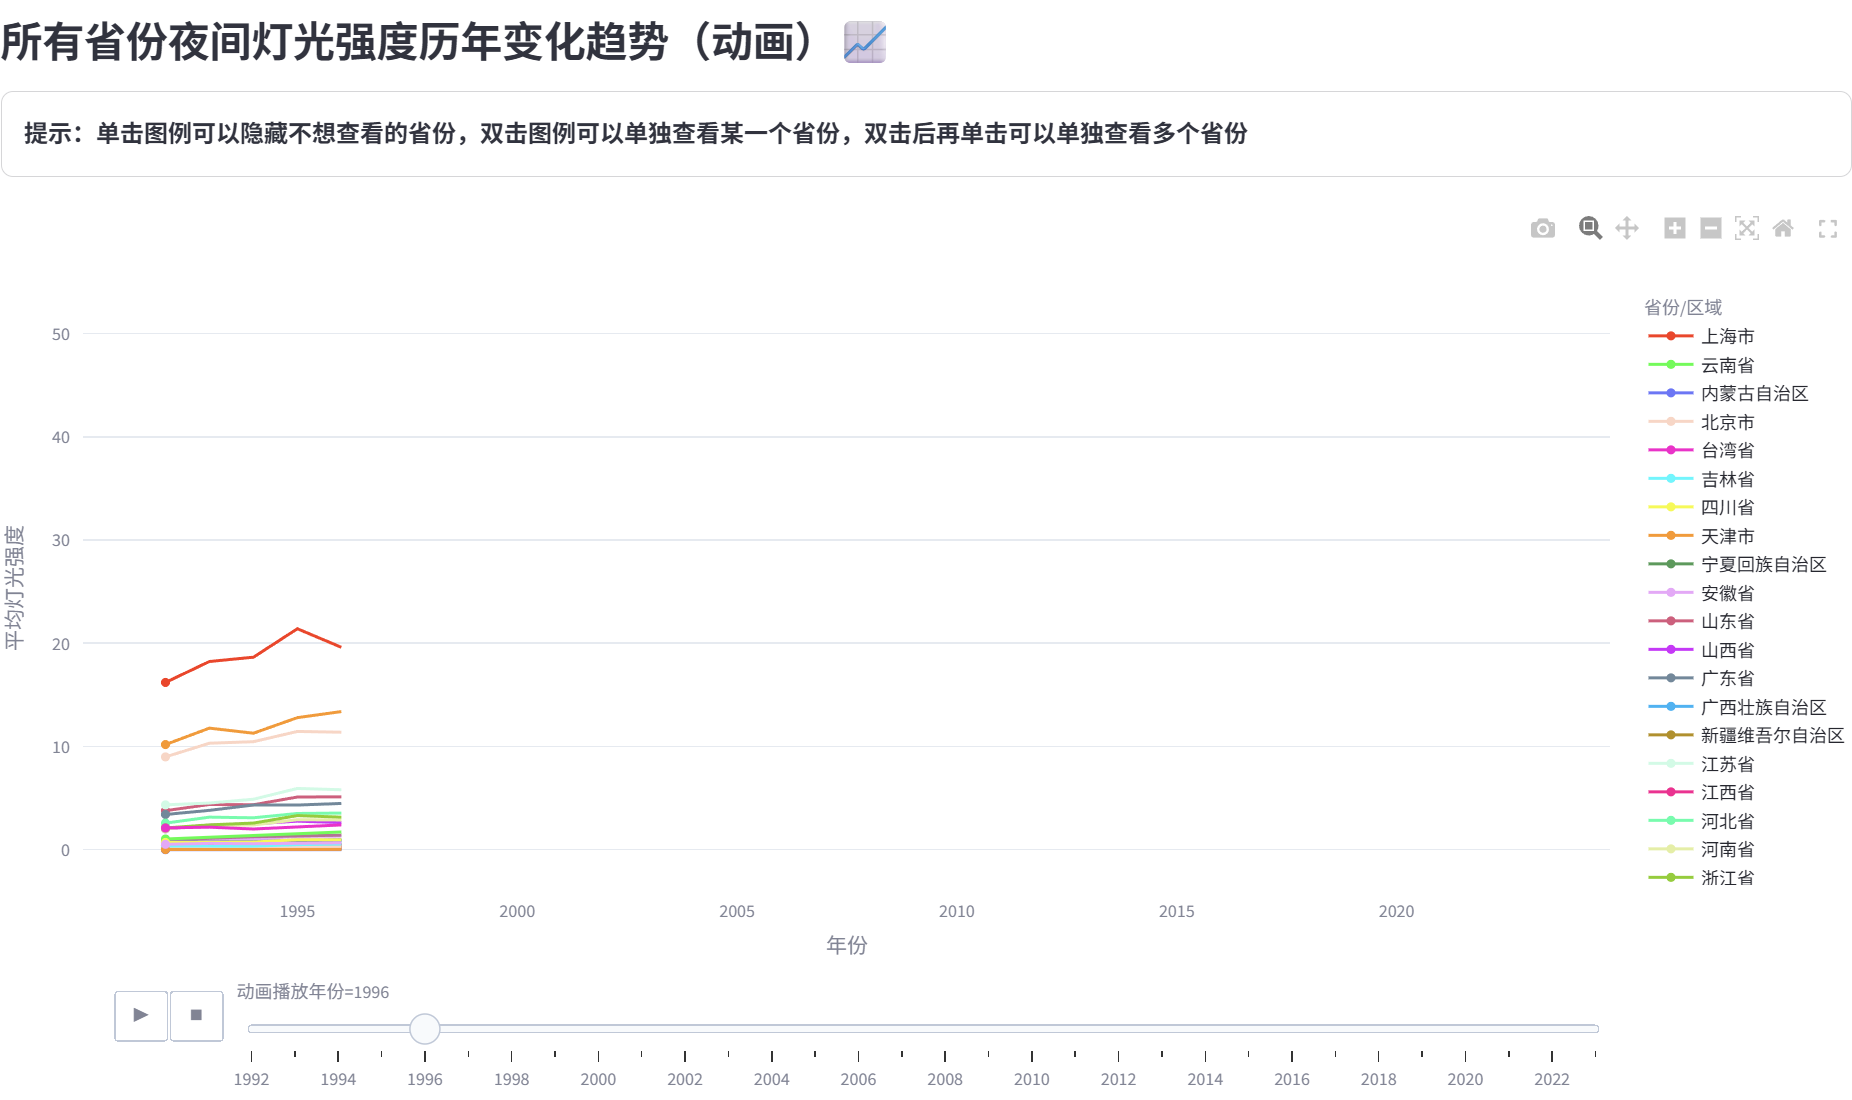
\includegraphics[width=\linewidth]{fig/plot_animation1.png}}
    \label{MLEDdet}
    \end{minipage}
    \quad
    \begin{minipage}{.45\linewidth}
    \centering
    \fbox{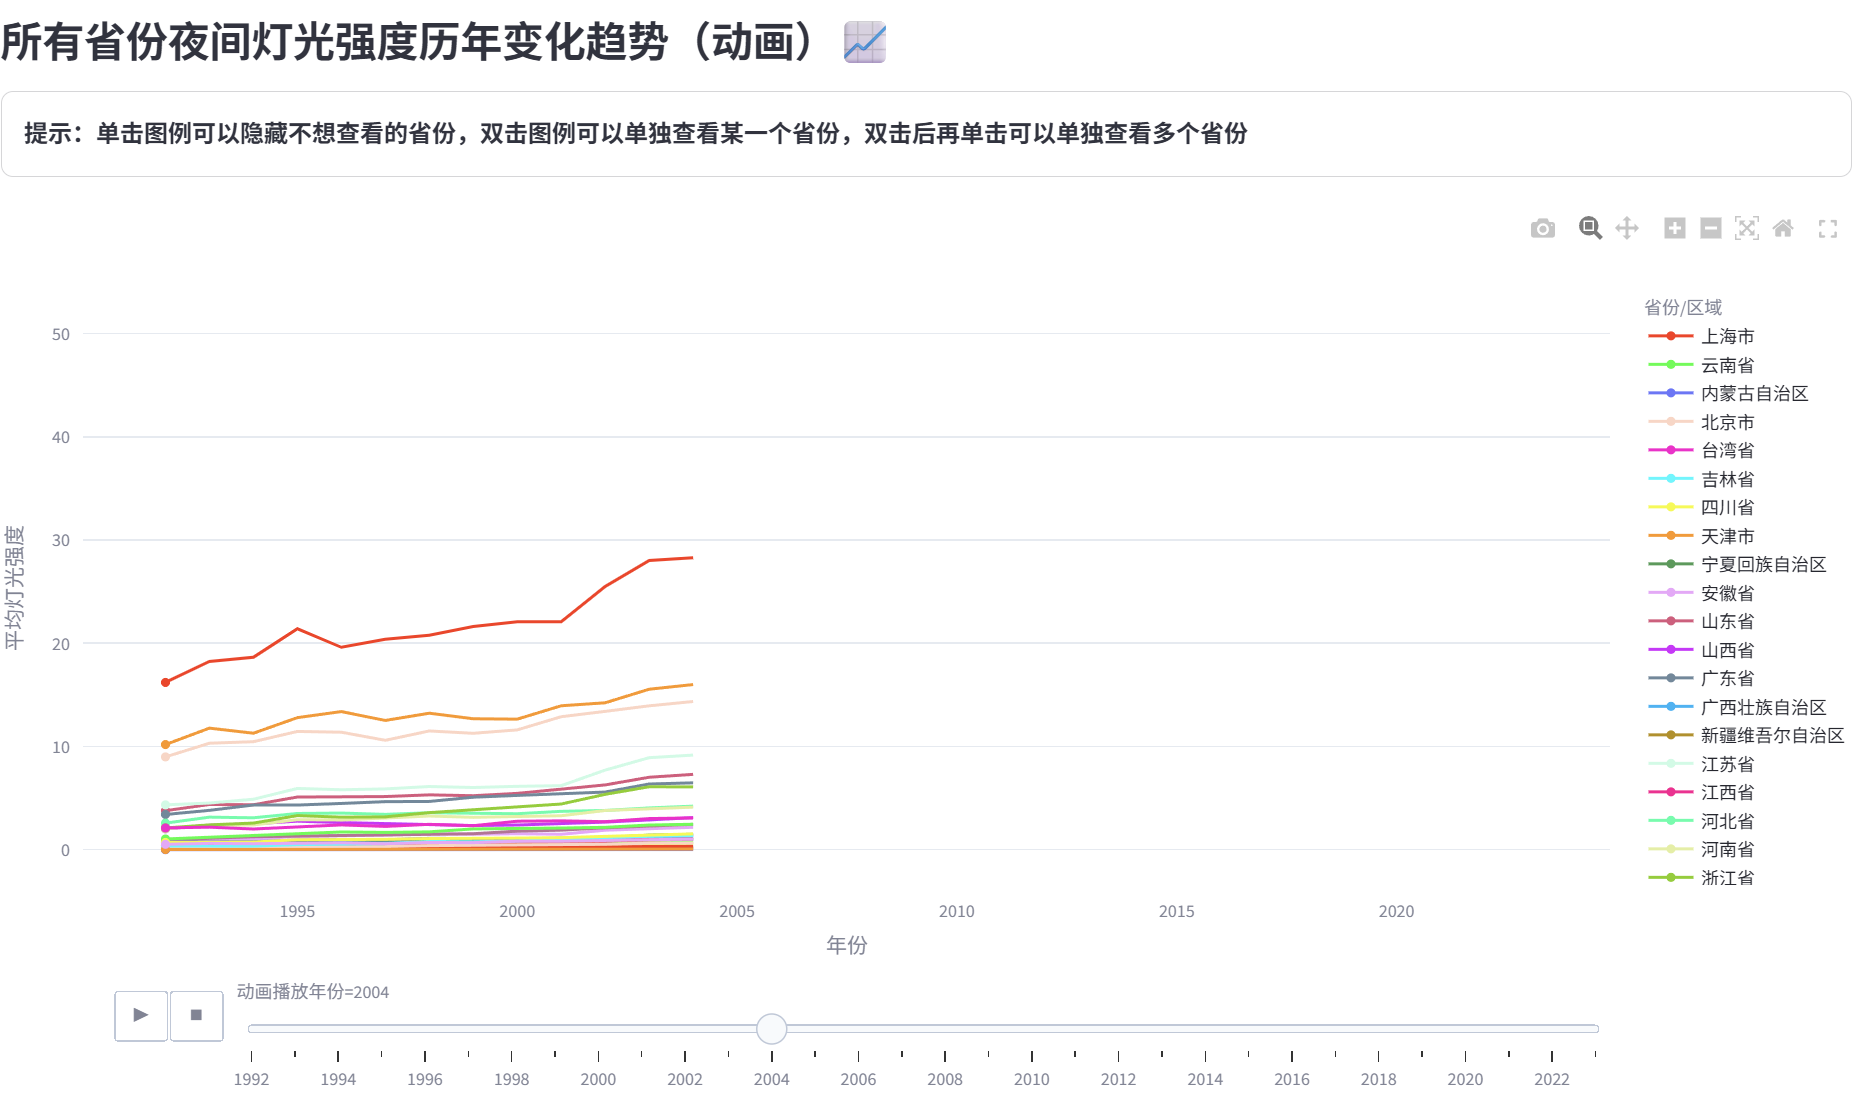
\includegraphics[width=\linewidth]{fig/plot_animation2.png}}
    \label{energydetPSK}
    \end{minipage}
    \begin{minipage}{.45\linewidth}
    \centering
    \fbox{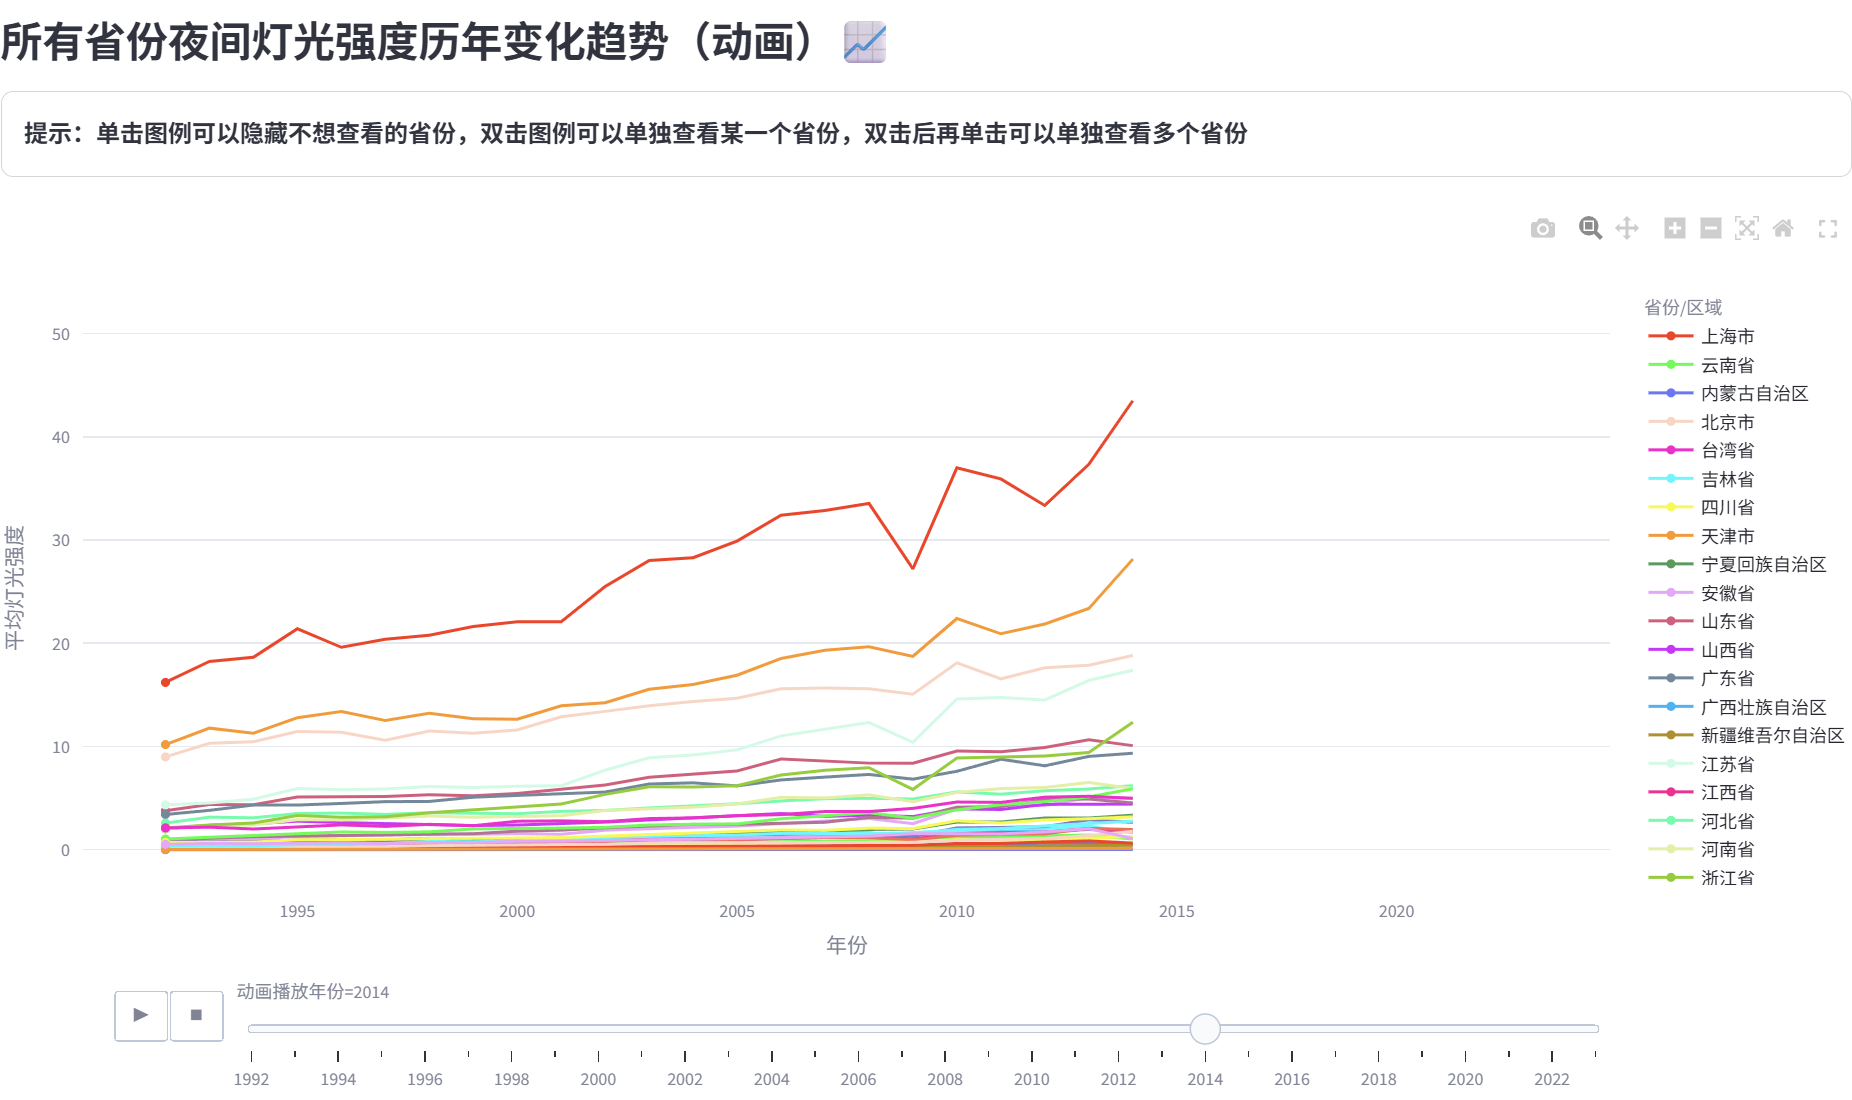
\includegraphics[width=\linewidth]{fig/plot_animation3.png}}
    \label{velcomp}
    \end{minipage}
    \quad
    \begin{minipage}{.45\linewidth}
    \centering
    \fbox{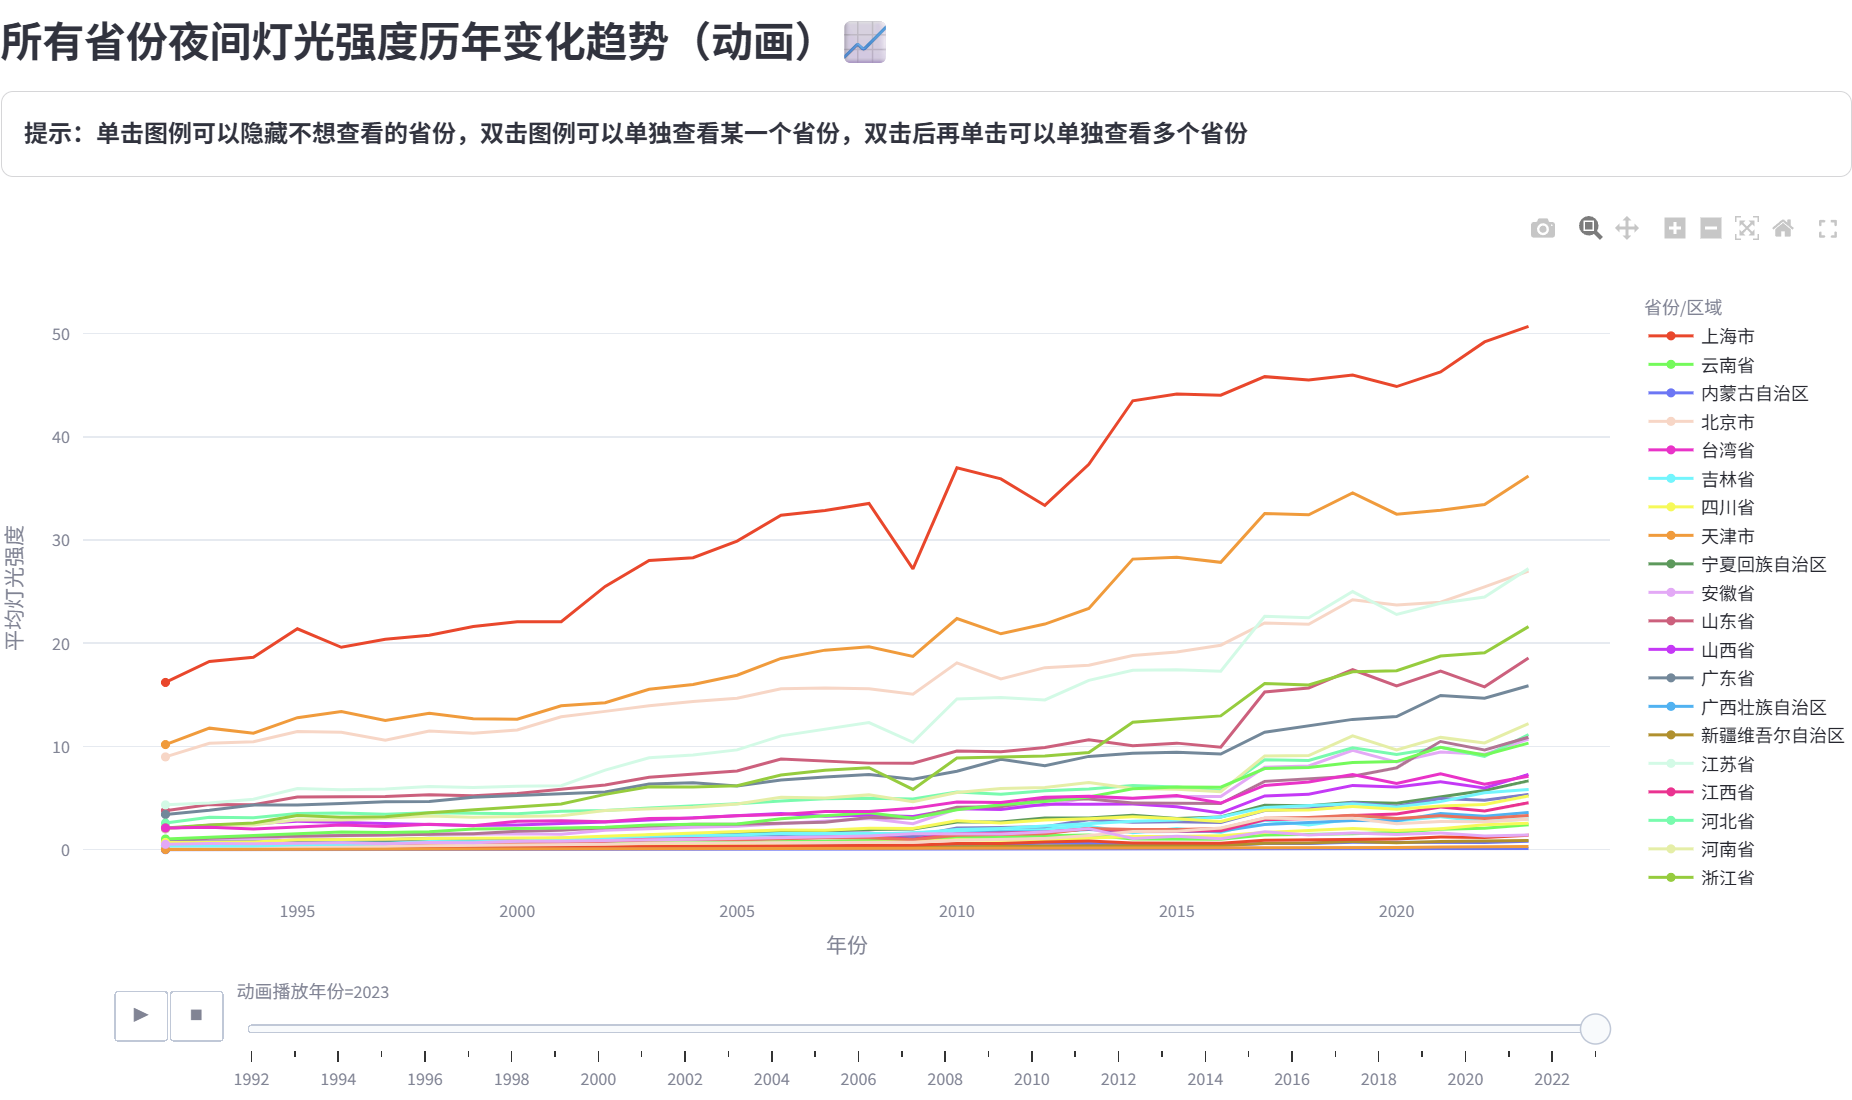
\includegraphics[width=\linewidth]{fig/plot_animation4.png}}
    \label{estcomp}
    \end{minipage}
    \caption{}
    \label{fig:roc}
    \end{figure}

    \item \textbf{2D/3D 视角切换与立体可视化}:
    \begin{itemize}
        \item 为了提供更具冲击力和直观性的数据展示方式,我还用了Pydeck库来创建一个3D立体图。
        \item 在3D视图中,每个省份的夜间灯光强度值被用作其地理边界在地图上拉伸的“高度”,从而将抽象的数据转化为具体的高度,非常直观。
        \item 用户还可以通过侧边栏的滑块实时调整3D拉伸的倍数,以获得最佳的视觉效果。
    \end{itemize}
    \begin{figure}[H]
        \centering
        \fbox{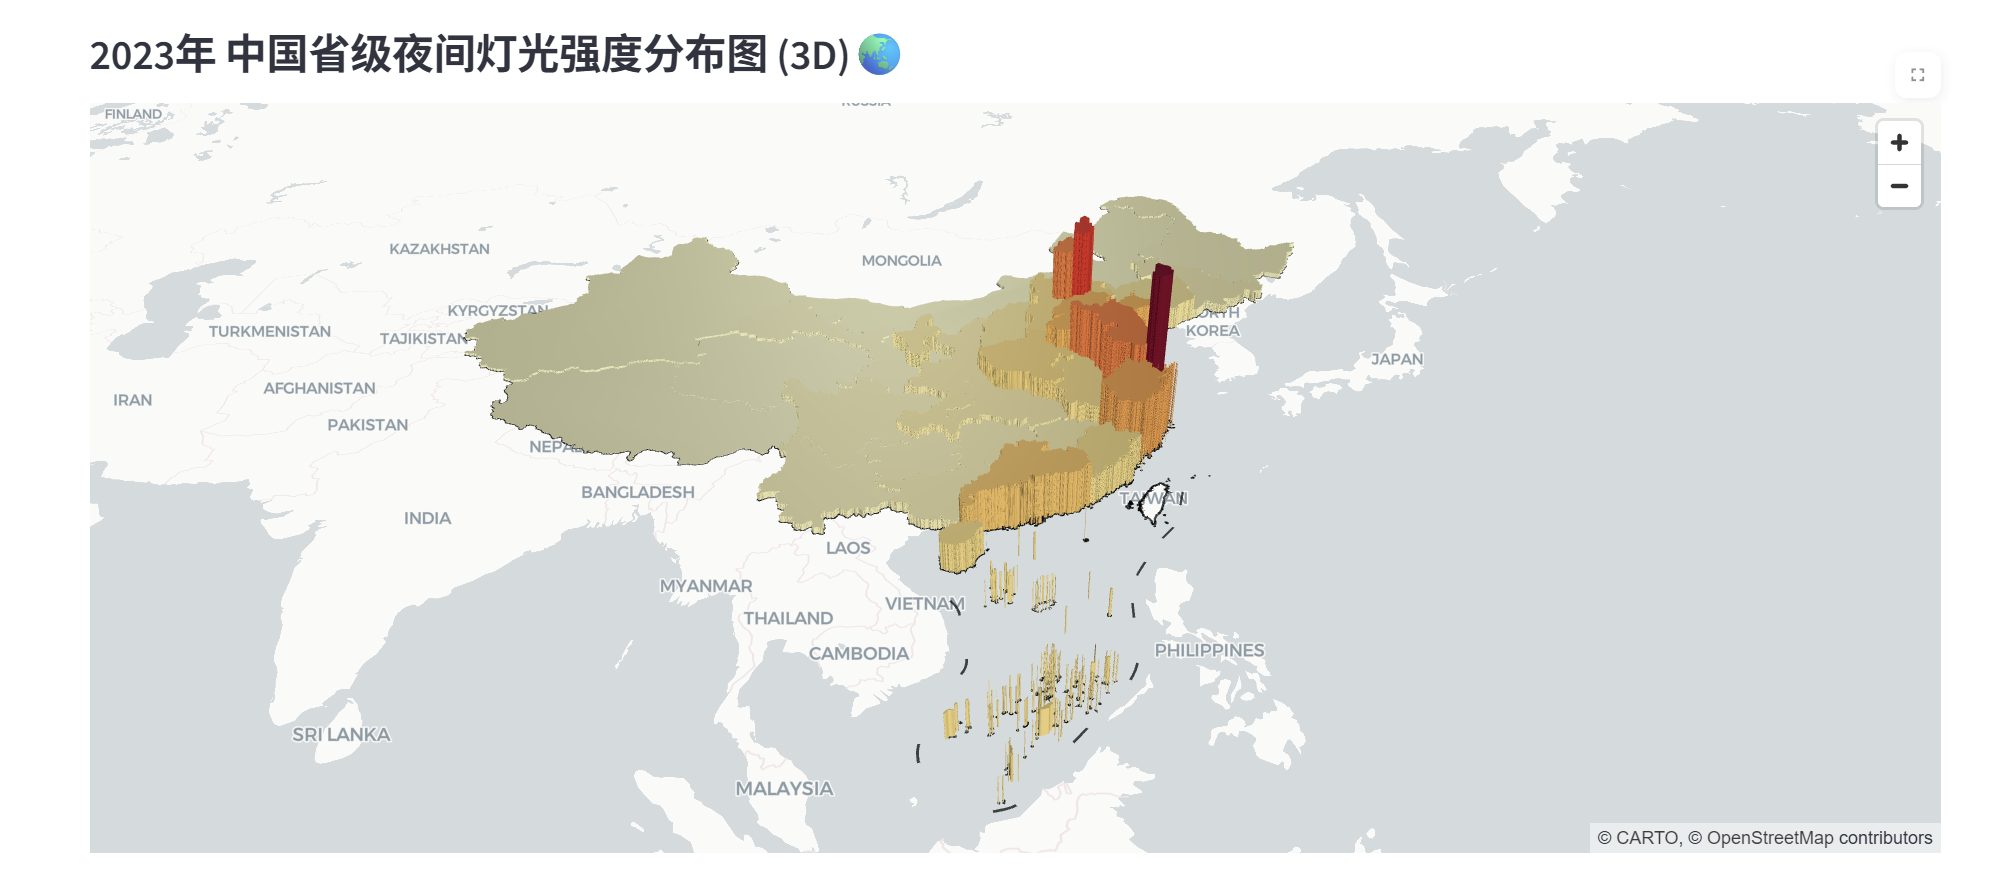
\includegraphics[width=0.8\textwidth]{fig/3d_map_example.png}} % 请将此处的图片路径替换为您3D地图的截图
        \caption{3D立体地图示例}
        \label{fig:3d_map_example}
    \end{figure}

\end{itemize}

\section{主要使用库}
本系统主要采用以下Python库:
\begin{itemize}
    \item \textbf{Streamlit}: 用于快速构建交互式Web应用程序的用户界面。
    \item \textbf{Geopandas和Pandas}: Geopandas用于处理地理空间数据,Pandas用于数据处理和分析。
    \item \textbf{Folium} 和 \textbf{Folium Plugins}: 用于创建2D交互式Leaflet地图,并实现标记簇、并排底图、流动线等高级功能。
    \item \textbf{Pydeck}: 用于创建高性能的3D地理空间可视化。
    \item \textbf{Plotly Express}: 用于生成高质量的交互式图表,尤其是本项目中的动画折线图。
    \item \textbf{Matplotlib}: 主要用于为Pydeck的3D地图提供颜色映射方案。
    \item \textbf{Rasterio} 和 \textbf{Rasterstats}: 用于读取原始GeoTIFF栅格数据并执行分区统计。
    \item \textbf{OS, glob, re}: 用于文件系统操作和正则表达式匹配,辅助数据文件的查找和管理。
\end{itemize}
\section{数据说明}
\subsection{数据来源与格式}
数据采用哈佛大学数据库的"An improved time-series DMSP-OLS-like data (1992-2024) in China by integrating DMSP-OLS and SNPP-VIIRS"\footnote{网址:https://dataverse.harvard.edu/dataset.xhtml?persistentId=doi:10.7910/DVN/GIYGJU}数据,即中国“类DMSP-OLS”1km 夜间灯光遥感数据集,格式是GeoTIFF。另外,我还使用了中国省级行政区划的Shapefile数据\footnote{网址:https://gaohr.win/site/blogs/2017/2017-04-18-GIS-basic-data-of-China.html}。
% 系统使用年度夜间灯光统计数据,这些数据预先处理并存储为Shapefile格式 (\texttt{.shp})。每个Shapefile文件对应一个特定年份的全国省级夜间灯光数据。
\subsection{数据处理流程}
\texttt{data\_preprocessing.py}、\texttt{province\_nightlight.py}和\texttt{cities\_nightlight.py}三个文件分别负责数据预处理和生成地图需要的Shapefile的生成。

\begin{itemize}
    \item \texttt{data\_preprocessing.py}的主要功能是;

\begin{enumerate}
    \item 由于原始数据中,2017年前包含港澳台地区的夜间灯光数据,但2017年后不再包含港澳台地区,因此需要对2017年后的数据进行处理,删除港澳台地区的夜间灯光数据。我在这里使用省级行政区划的Shapefile数据删去港澳台地区后,对GeoTIFF数据进行掩膜裁剪。
    \item 原始数据中一部分的NoData值是-128,有一些是未定义,为了后续处理方便,我将这些NoData值统一替换为-128。
    \item 将处理完的图像命名为“\texttt{clipped\_原文件名称}”,并保存到\texttt{region\_excluded\_tiffs}目录下。
\end{enumerate}
    \item \texttt{provinces\_nightlight.py}和\texttt{cities\_nightlight.py}的主要功能是:

    \begin{enumerate}
        \item 在已有的省级区划和市级区划Shapefile的基础上,添加夜间灯光数据列。
        \item 夜间灯光数据的计算整合方式是使用Rasterstats包中的分区运算(Zonal Statistics)方法,对每个省份和市的像元值总和再除以该省份所占的像元数。
        \item 最后将处理后的Shapefile文件统一命名为,保存到特定的目录下。
    \end{enumerate}
\end{itemize}





\section{主程序代码结构概览}

\begin{enumerate}

    \item \textbf{定义辅助函数} (部分带有 \texttt{@st.cache\_data}来缓存结果,可以减少加载时间,虽然我感觉没啥效果)
        \begin{itemize}
            \item \texttt{load\_yearly\_data(shp\_path)}: 加载Shapefile文件生成GeoDataFrame,并且把澳门的英文修正为Macao。
            \item \texttt{load\_china\_boundary(shp\_path)}: 加载中国国界的线要素Shapefile。
            \item \texttt{generate\_shapefile\_dict(directory)}: 扫描指定目录,根据文件名模式提取年份,并为每年生成一个包含对应Shapefile路径和灯光数据列名的字典。
            \item \texttt{generate\_shapefile\_dict\_for\_cities(directory)}:和上一个函数类似,但用于市级Shapefile数据,主要用于市级灯光强度标记簇的生成。
            \item \texttt{generate\_yearly\_ntl\_dataframe(year\_dict, province)}: 主要用来接收上一步生成的字典和省份字段名,遍历所有年度的Shapefile,并将所有省份、所有年份的灯光数据整合到一个DataFrame中。
        \end{itemize}
    
    \item \textbf{Streamlit侧边栏配置}
        \begin{itemize}
            \item 调用 \texttt{generate\_shapefile\_dict} 获取所有可用的年度数据信息 (\texttt{year\_dict\_provinces})。
            \item 根据 \texttt{year\_dict\_provinces} 生成年份字典,并创建一个下拉菜单(\texttt{st.sidebar.selectbox}),用户可以选择要在Folium地图上显示哪一年的数据 (\texttt{selected\_year})。
            \item 根据用户选择的年份,从 \texttt{year\_dict\_provinces} 中获取对应的Shapefile路径 (\texttt{selected\_shp\_path\_provinces}) 和灯光数据列名\\ (\texttt{selected\_ntl\_column})。
            \item 创建一个包含多种Brewer颜色方案的列表,并提供一个配色方案下拉菜单 (\texttt{selected\_color\_scheme})。
            \item 使用 \texttt{st.sidebar.info} 显示当前选定的年份、数据文件、灯光列和配色方案。
            \item 提供勾选框 (\texttt{st.sidebar.checkbox}) 让用户选择是否在地图上叠加标记簇 (\texttt{show\_cluster\_option}),是否使用并排比较的底图 (\texttt{show\_layer\_option}),以及是否添加国界流动线 (\texttt{show\_antpath\_option})。
            \item 提供一个单选框(\texttt{st\.sidebar\.radio})让用户在“2D平面视图”和“3D立体视图”之间切换。
            \item 根据选择的视图,条件性地显示平面地图的分级数量滑块或3D地图的高度拉伸倍数滑块。
        \end{itemize}

 \begin{figure}[H]
    \centering % 整个 figure 环境居中
    \begin{subfigure}{0.24\linewidth} % 调整宽度,例如 0.24\linewidth
        \centering
        \fbox{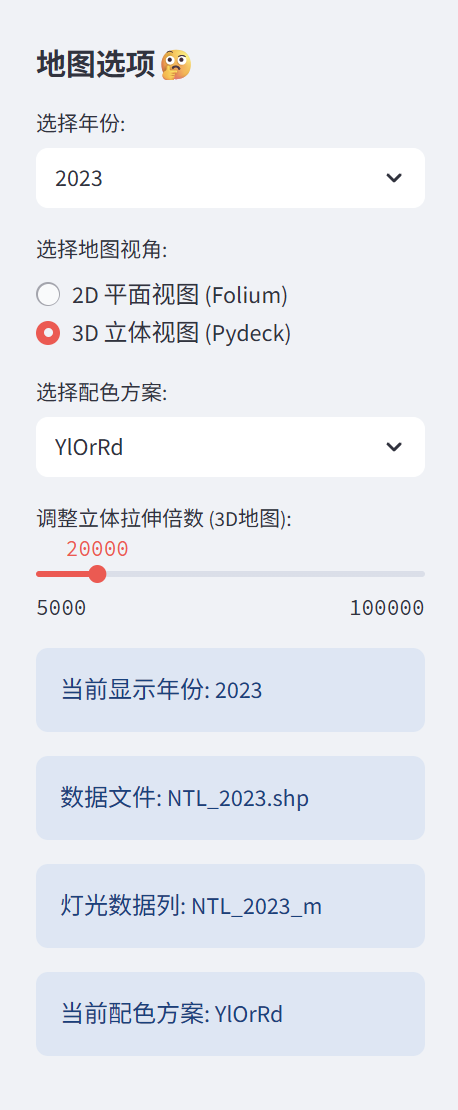
\includegraphics[width=0.7\textwidth]{fig/sidebar_overview1.png}}
        \caption{侧边栏概览(选择3D)} 
        \label{fig:sidebar_example}
    \end{subfigure} % 使用 \hfill 均匀分布空白
    \begin{subfigure}{0.24\linewidth} % 调整宽度
        \centering
        \fbox{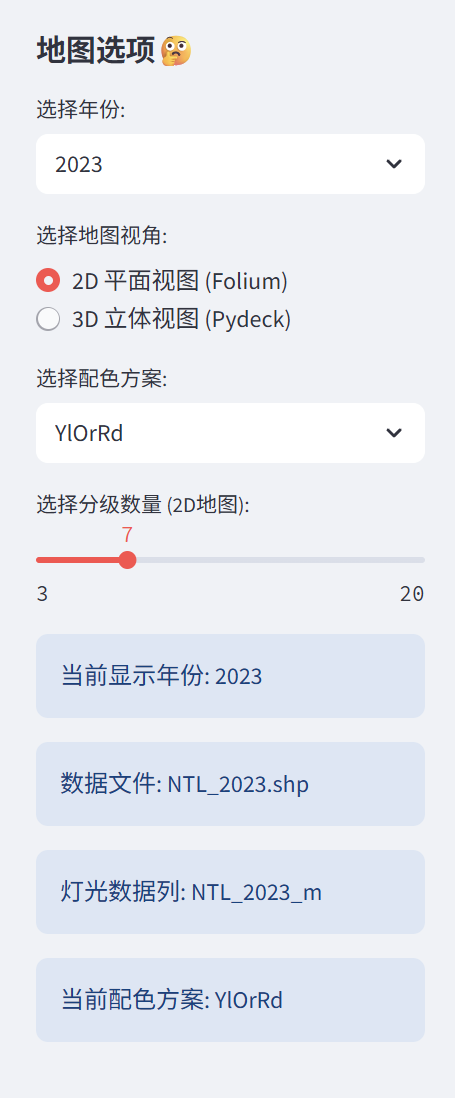
\includegraphics[width=0.7\textwidth]{fig/sidebar_overview2.png}}
        \caption{(选择2D)}
        \label{fig:sidebar_options}
    \end{subfigure} % 使用 \hfill 均匀分布空白
    \begin{subfigure}{0.24\linewidth} % 调整宽度
        \centering
        \fbox{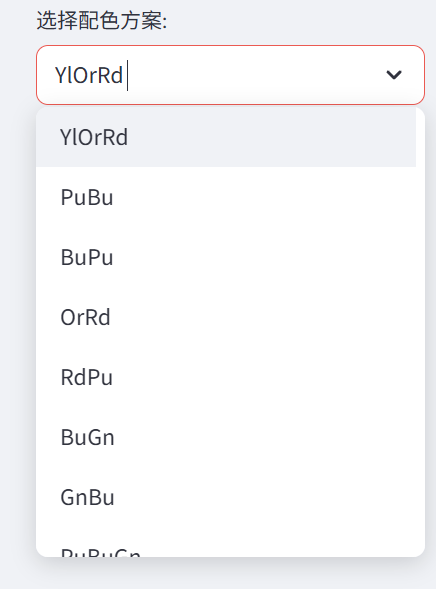
\includegraphics[width=0.7\linewidth]{fig/sidebar_chroma.png}}
        \caption{配色方案选择}
        \label{fig:sidebar_chroma}
    \end{subfigure} % 使用 \hfill 均匀分布空白
    \begin{subfigure}{0.24\linewidth} % 调整宽度
        \centering
        \fbox{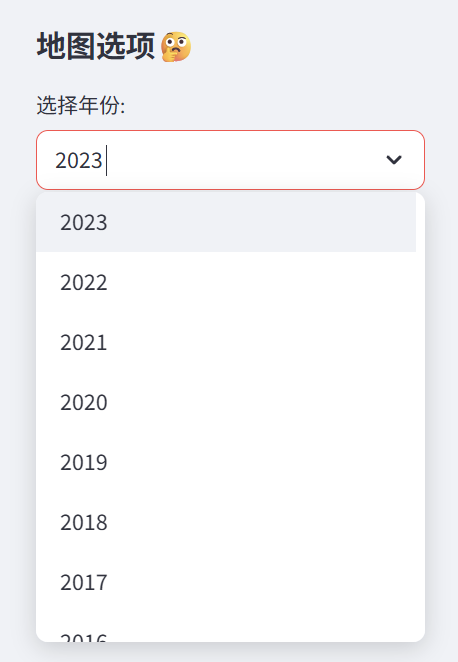
\includegraphics[width=0.7\linewidth]{fig/sidebar_years.png}} % 这里图片宽度可能需要调整以适应 subfigure 宽度
        \caption{年份下拉菜单}
        \label{fig:sidebar_years}
    \end{subfigure}
    \caption{Streamlit侧边栏配置}
    \label{fig:sidebar_config}
\end{figure}


    \item \textbf{加载和预处理当前选定年份的地图数据}
        \begin{itemize}
            \item 初始化进度条 (\texttt{st.progress}) 和可选的小游戏显示 (\texttt{st.components.v1.html})。
            \item 调用 \texttt{load\_yearly\_data} 加载当前 \texttt{selected\_year} 对应的省级灯光数据 (\texttt{gdf\_provinces\_yearly})。
            \item 调用 \texttt{load\_china\_boundary} 加载中国国界数据 (\texttt{china\_boundary})。
            \item 对加载的 \texttt{gdf\_provinces\_yearly} 中的灯光数据列进行数值类型转换。
            \item 计算当前年份各省灯光强度占全国总量的百分比,替换NaN值为0,并将结果作为一个新列添加到\\ \texttt{gdf\_provinces\_yearly}中,列名为“\texttt{NTL\_年份\_占比}”。
        \end{itemize}

    \item \textbf{创建和配置核心Folium地图对象 (\texttt{m})}
        \begin{itemize}
            \item 使用 \texttt{folium.Map()} 初始化地图,设置默认的中心点、缩放级别和底图样式。
            \item 从 \texttt{gdf\_provinces\_yearly} 准备用于Choropleth图层的数据 (\texttt{data\_for\_map})。
            \item 创建并添加 \texttt{folium.Choropleth} 图层到地图 \texttt{m},根据用户选择的年份 (\texttt{selected\_year})、配色方案 \\(\texttt{selected\_color\_scheme}) 和灯光数据列 (\texttt{selected\_ntl\_column}) 对各省进行颜色填充。设置图例名称、高亮等属性。
            \item 为Choropleth图层添加 \texttt{folium.GeoJsonTooltip},以便鼠标悬停时显示省份名称、当年灯光强度和占比信息。
                \begin{figure}[H]
                    \centering
                    \fbox{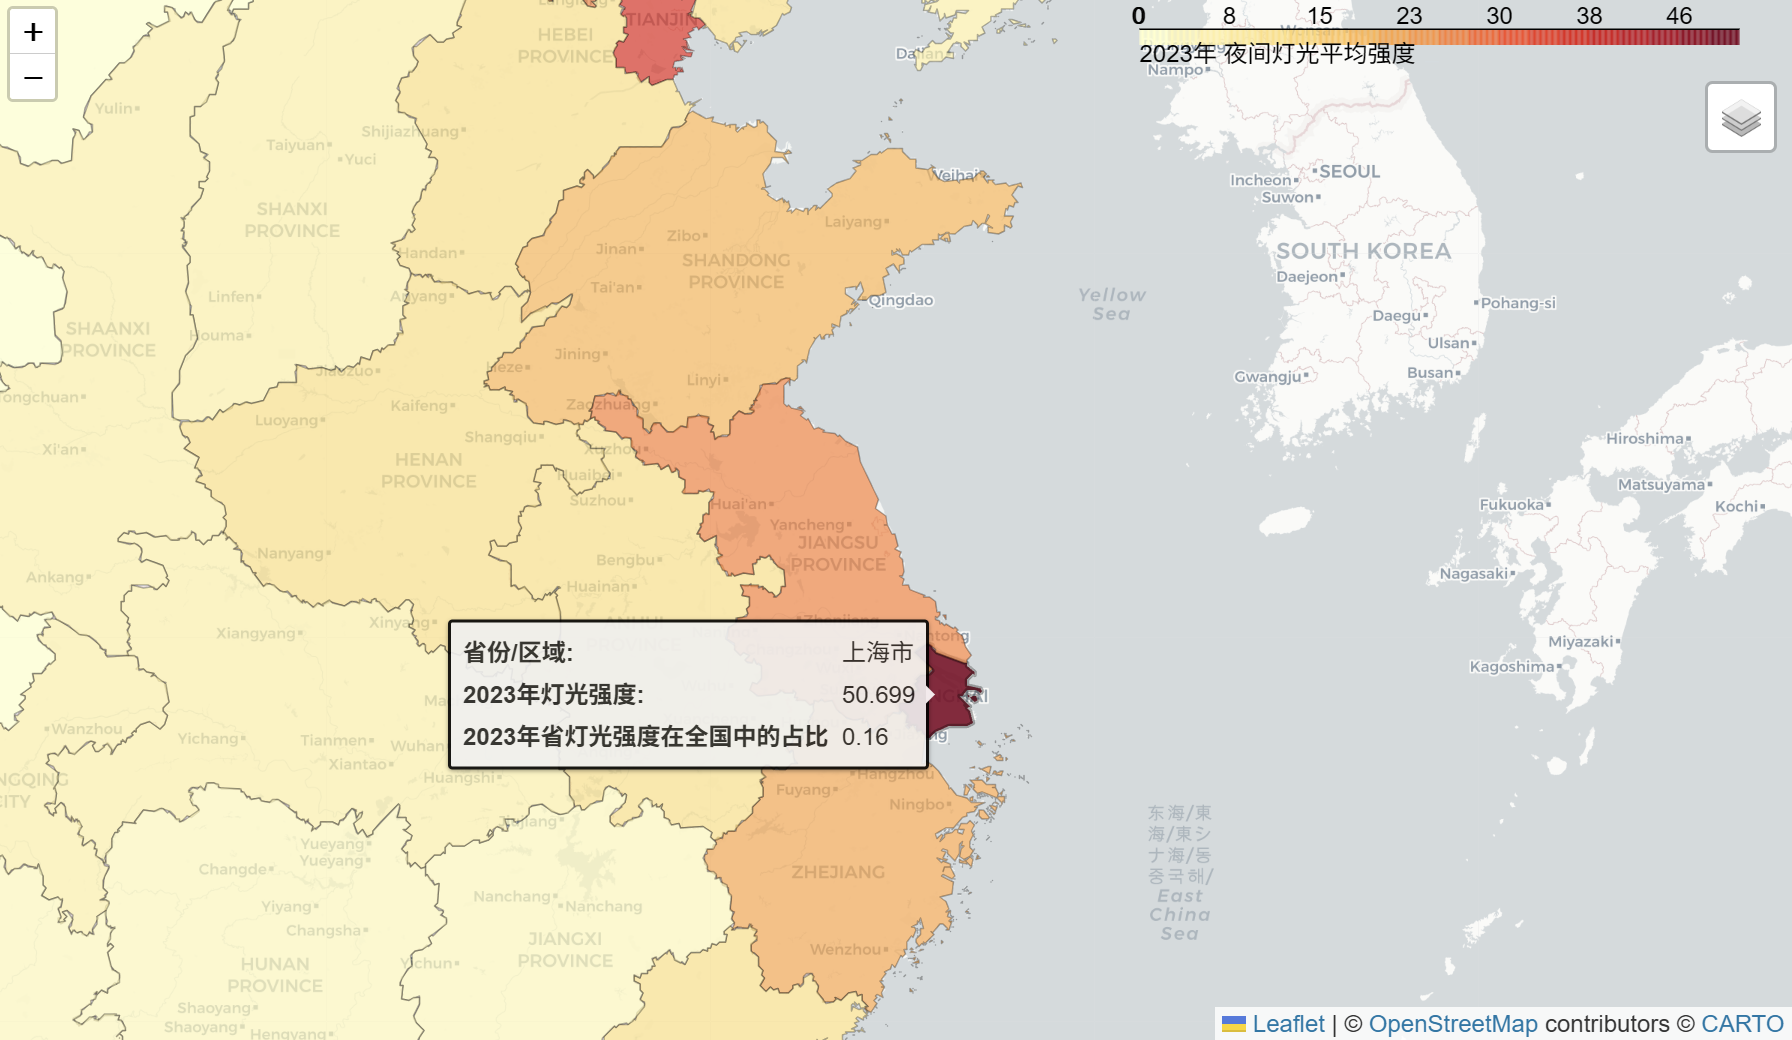
\includegraphics[width=0.7\textwidth]{fig/geojson.png}}
                    \caption{Tooltip信息示例}
                    \label{fig:choropleth_example}
                \end{figure}
            \item 在这些过程进行的时候更新进度条,方便用户了解加载状态。
        \end{itemize}

    \item \textbf{根据用户在侧边栏的选择,条件性地添加额外的Folium插件图层到地图 \texttt{m}}
        \begin{itemize}
            \item 如果勾选 \texttt{show\_cluster\_option}:
                \begin{itemize}
                    \item 从 \texttt{gdf\_cities\_yearly} 提取市级质心和灯光强度值,准备标记簇数据点。
                    \item 创建并添加 \texttt{MarkerCluster}。
                \end{itemize}
                \begin{figure}[H]
                    \centering
                    \fbox{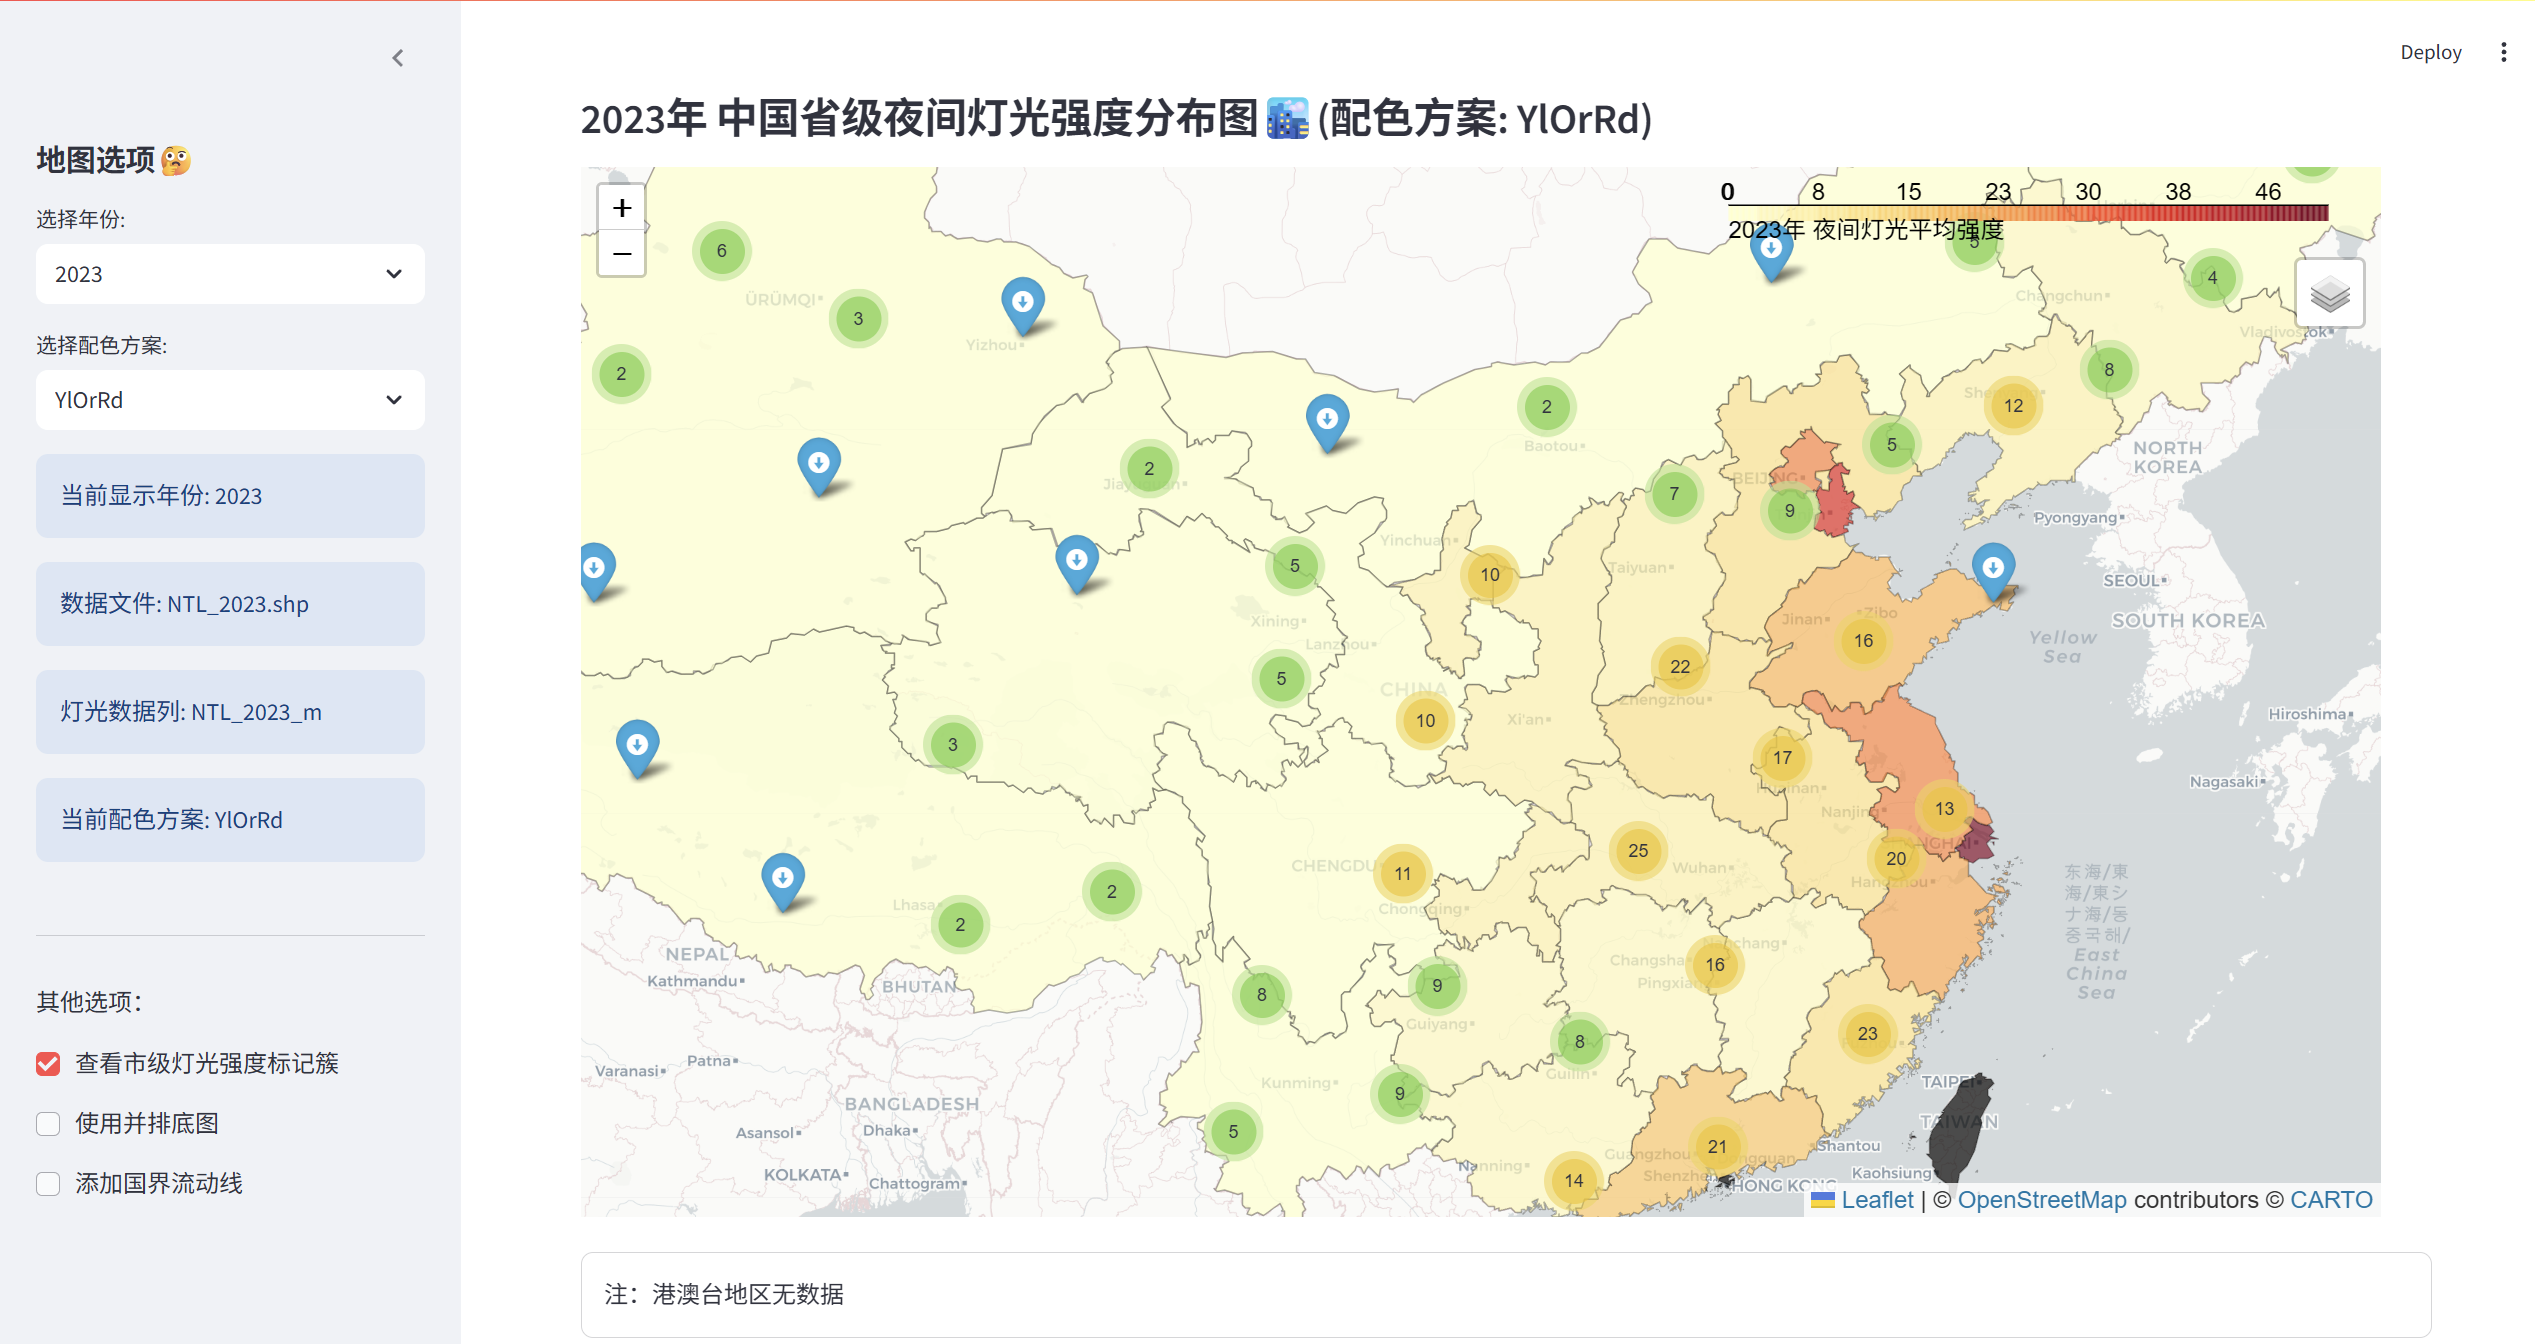
\includegraphics[width=0.7\textwidth]{fig/markers_example.png}}
                    \caption{市级灯光强度标记簇示例}
                    \label{fig:marker_cluster_example}
                \end{figure}
            \item 如果勾选 \texttt{show\_layer\_option}:
                \begin{itemize}
                    \item 创建左右两个不同的 \texttt{folium.TileLayer} (例如 \texttt{openstreetmap} 和 \texttt{cartodbpositron})。
                    \item 将这两个瓦片图层添加到地图 \texttt{m}。
                    \item 创建并添加 \texttt{folium.plugins.SideBySideLayers}。
                \end{itemize}
                \begin{figure}[H]
                    \centering
                    \fbox{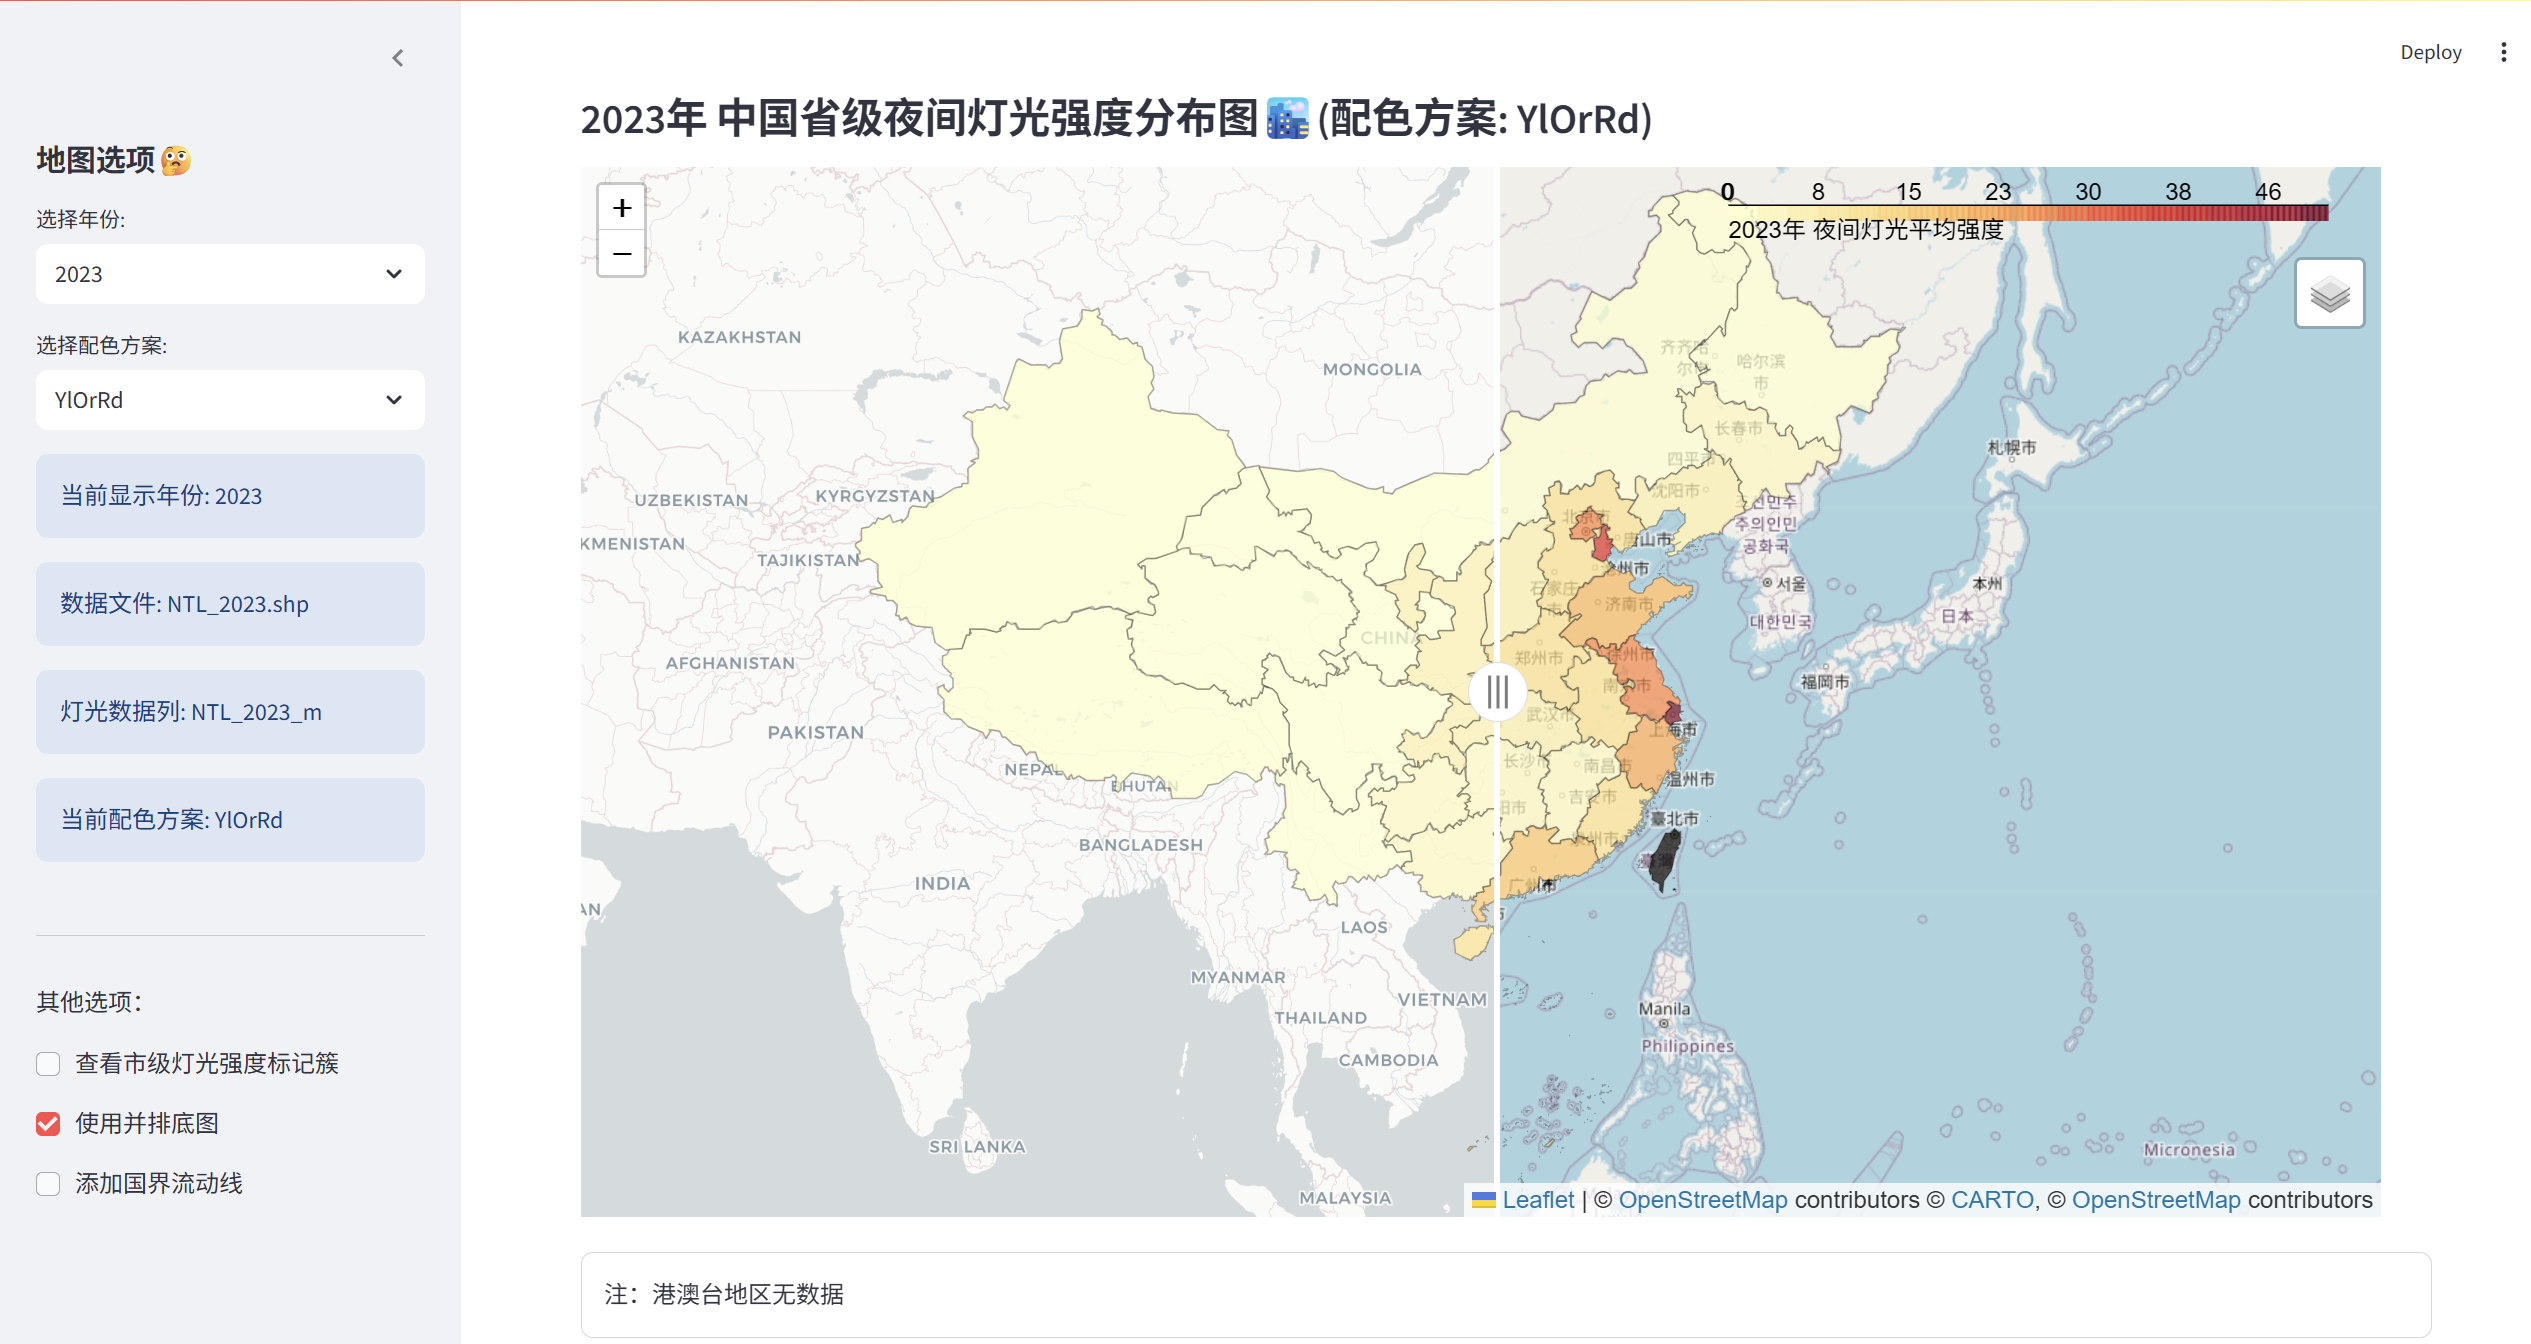
\includegraphics[width=0.7\textwidth]{fig/sidebyside_example.png}}
                    \caption{并排底图示例}
                    \label{fig:sidebyside_example}
                \end{figure}
            \item 如果勾选 \texttt{show\_antpath\_option}:
                \begin{itemize}
                    \item 确保国界数据 (\texttt{china\_boundary}) 的坐标系正确。
                    \item 从国界数据的几何对象中提取坐标点列表。
                    \item 创建并添加 \texttt{folium.plugins.AntPath}。
                \end{itemize}
                \begin{figure}[H]
                    \centering
                    \fbox{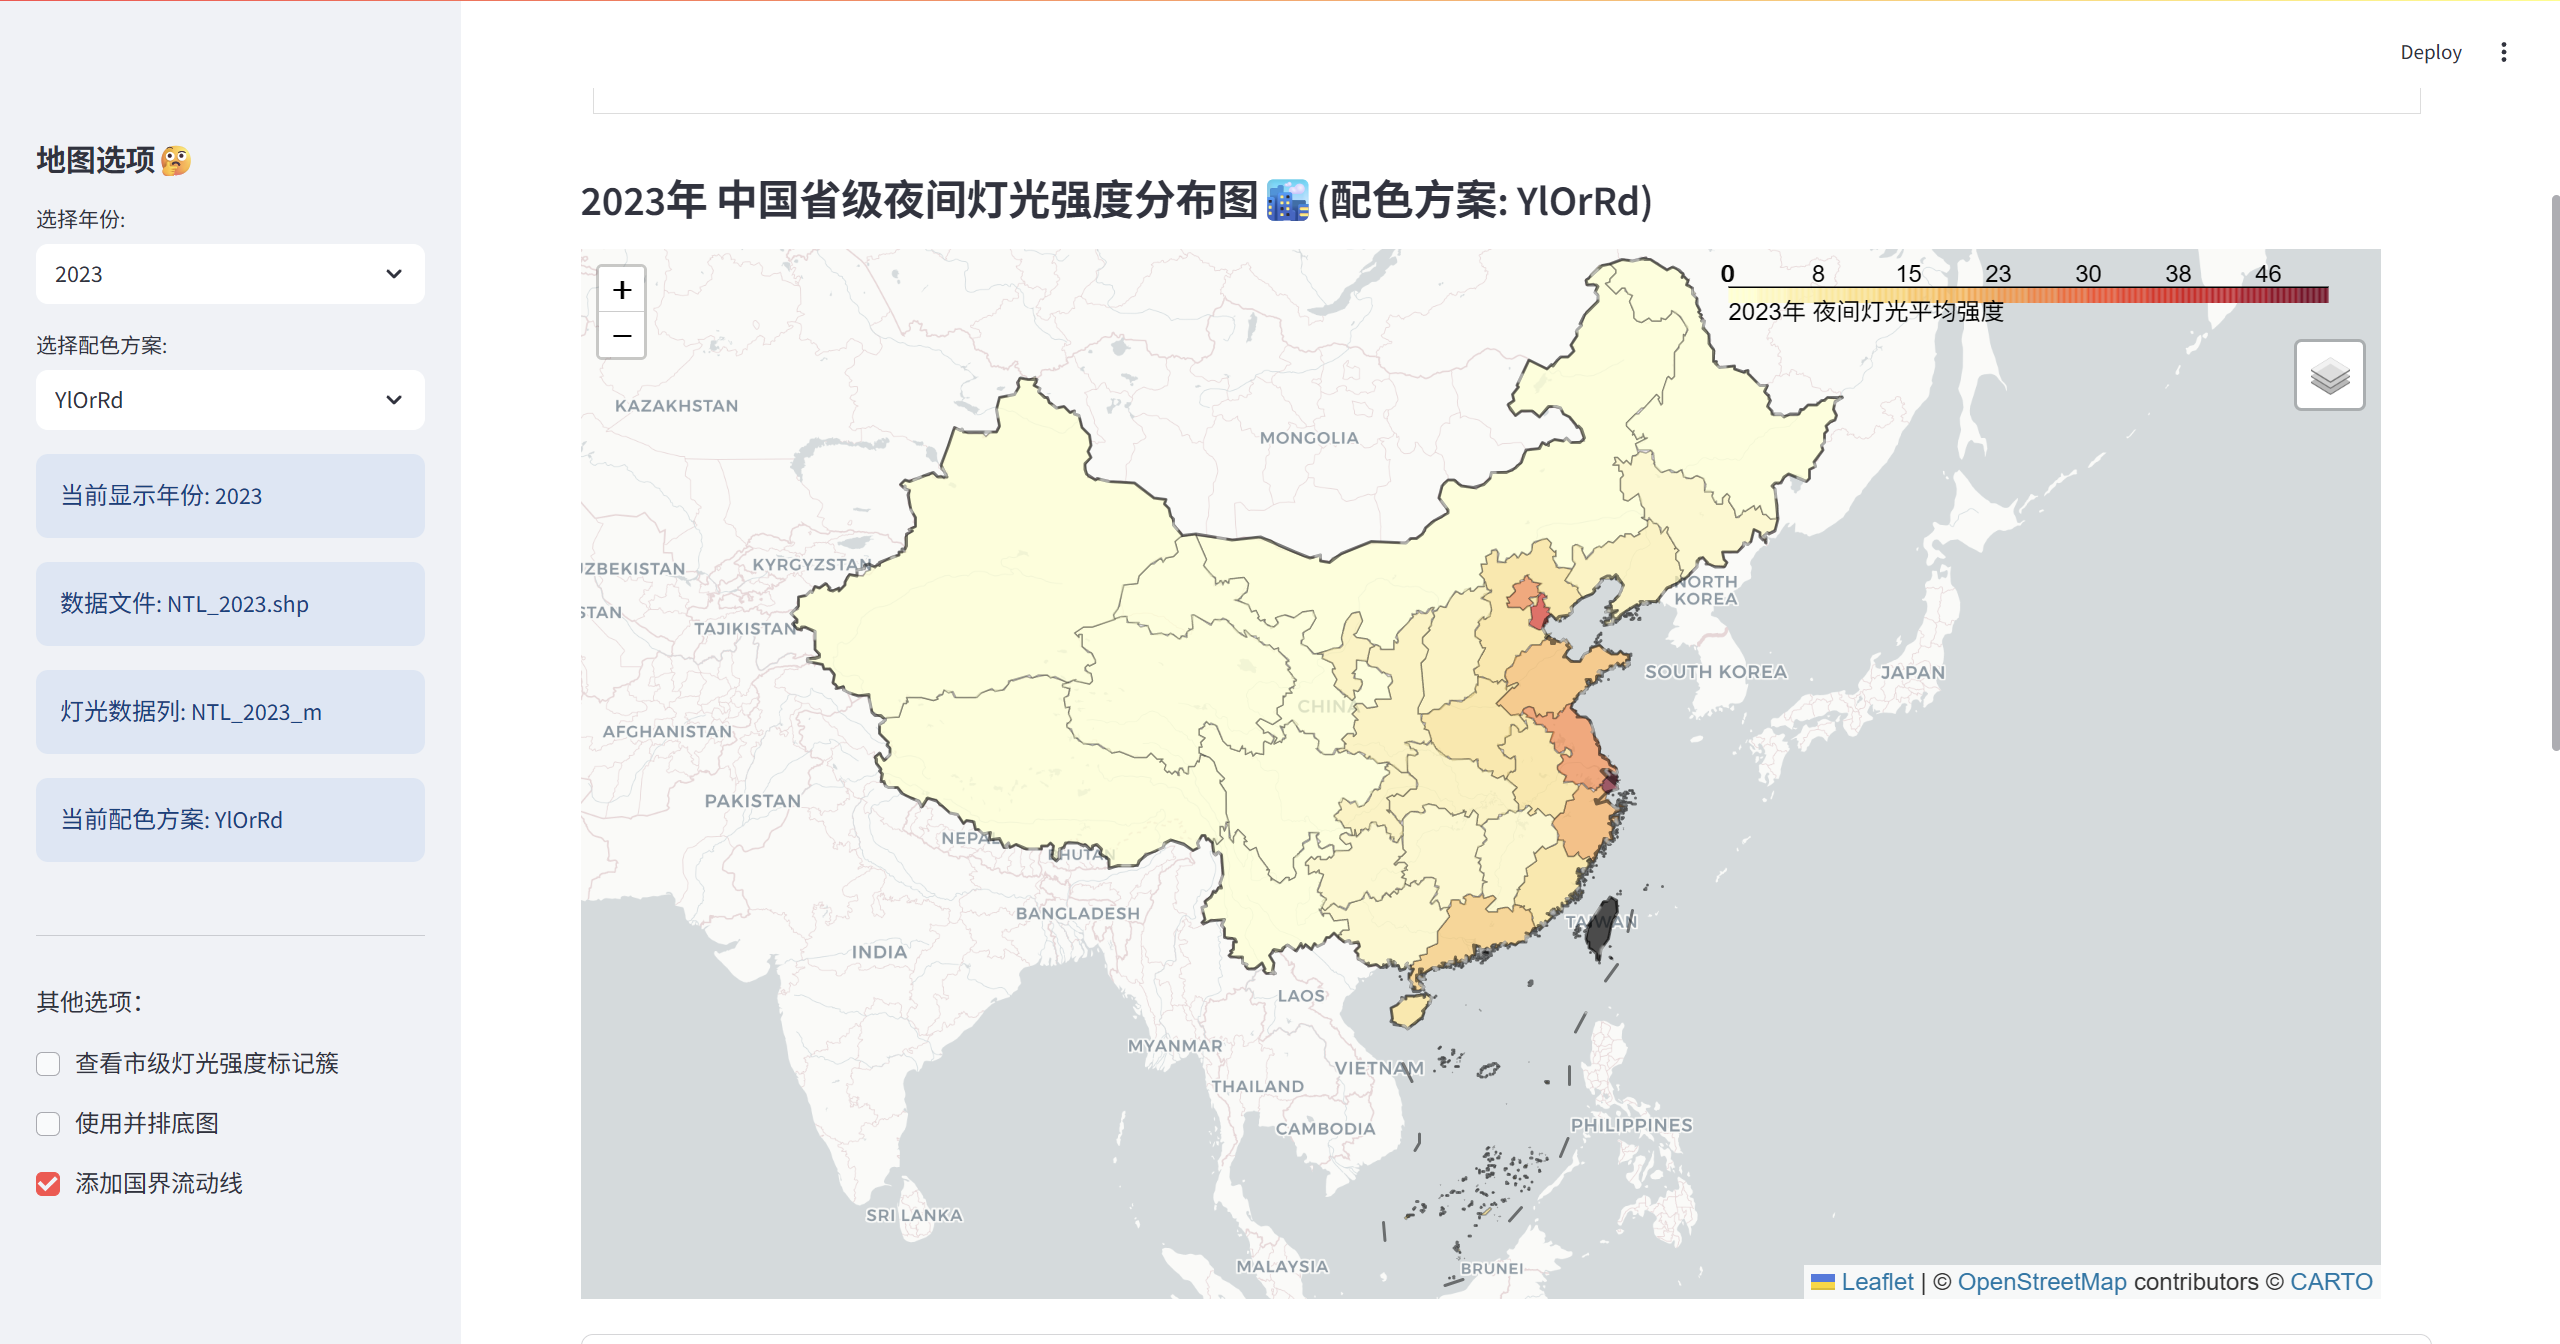
\includegraphics[width=0.7\textwidth]{fig/overall_map.png}}
                    \caption{国界流动线示例}
                    \label{fig:antpath_example}
                \end{figure}
            \item 调用 \texttt{folium.LayerControl().add\_to(m)},允许用户切换不同图层的可见性。
        \end{itemize}

    \item \textbf{在Streamlit中显示地图}

    
        \begin{itemize}
        \item \textbf{如果选择2D视图}:
            \begin{itemize}
                \item 加载并预处理当前年份的省级和市级灯光数据。
                \item 创建Folium地图对象(\texttt{m})。
                \item 创建并添加核心的\texttt{folium.Choropleth}分层设色图层。
                \item 为其添加\texttt{folium.GeoJsonTooltip}以显示悬停信息。
                \item 根据用户勾选,条件性地添加\texttt{MarkerCluster}, \texttt{SideBySideLayers}, \texttt{AntPath}等插件图层。
                \item 添加图层控制器(\texttt{folium.LayerControl})。
                \item 使用\texttt{st\_folium()}将地图渲染到页面。
                \item 加载完毕后,清空进度条,显示气球 \texttt{st.balloons()}效果。
            \end{itemize}
        \item \textbf{如果选择3D视图}:
            \begin{itemize}
                \item 加载当前年份的省级灯光数据。
                \item 准备Pydeck数据\textbf{(非常重要的一步,花了我很长时间来解决)}:
                    \begin{itemize}
                        \item 对GeoDataFrame使用\texttt{.explode()}方法,将\texttt{MultiPolygon}几何体转换为简单的\texttt{Polygon},以解决Pydeck的渲染问题。
                        \item 手动创建一个符合Pydeck格式的坐标列(\texttt{'coordinates'})。
                        \item 基于灯光强度值和用户选择的配色方案,为每个多边形进行亮度拉伸和颜色分配。
                    \end{itemize}
                \item  使用\texttt{pdk.Layer()}创建3D图层,其中\texttt{extruded=True}开启3D效果,\texttt{get\_elevation}使用灯光强度值作为高度。
                \item 将所有图层和初始视角(\texttt{pdk.ViewState})组合成一个\texttt{pdk.Deck}对象,并使用\texttt{st.pydeck\_chart()}进行渲染。
                \item 加载完毕后,清空进度条,显示气球 \texttt{st.balloons()}效果。
            \end{itemize}
    \end{itemize}
    

    \item \textbf{生成并显示所有省份历年灯光强度变化的Plotly动态折线图}
        \begin{itemize}
            \item 调用 \texttt{generate\_yearly\_ntl\_dataframe} 函数,传入 \texttt{year\_dict\_provinces}和省份字段名,生成包含所有年份、所有省份灯光数据的 \texttt{consolidated\_df}。
            \item 对 \texttt{consolidated\_df} 进行数据类型转换 (年份转为数值型) 和排序 (按年份、省份)。
            \item 创建累积数据帧 (\texttt{cumulative\_plot\_df}): 为了实现Plotly动画的“拖尾效果”,遍历每个唯一且排序后的年份。对于每个动画帧年份,从 \texttt{consolidated\_df} 中筛选出所有小于等于该年份的数据,并为这些数据添加一个动画帧ID列(其值为当前动画帧年份)。最后,将所有这些为各帧准备的子DataFrame合并。
            \item 设置图表区域的子标题 (\texttt{st.subheader}) 和用户提示信息 (\texttt{st.container().write()})。
            \item 使用 \texttt{st.spinner} 显示“正在生成动画折线图”的提示。
            \item 使用 \texttt{px.line()} 函数创建折线图 (\texttt{fig\_all\_provinces}),其中实现动画最重要的参数是\texttt{animation\_frame},这里我设置为\texttt{"animation\_frame\_id"},从而实现每年对应一个帧。
            \item 设置Plotly重要参数,以确保拖尾效果正确渲染\footnote{参数设置参考:https://stackoverflow.com/questions/70523979/how-to-create-an-animated-line-plot-with-ploty-express}。
        \end{itemize}

\end{enumerate}

\section{总结}

本次《软件工程与GIS开发》课程大作业中,我设计了一个具有多个功能、交互性强的中国年度夜间灯光强度可视化分析Web应用。这个项目以Streamlit为前端框架,后端集成了许多地理空间数据处理库,并融合了Folium、Pydeck和Plotly Express三种可视化库。

在本次开发过程中,我也遇到并解决了一系列挑战:
\begin{itemize}
    \item 在处理数据的过程中,我发现原始数据中存在一些NoData值不一致的问题,有一些GeoTIFF文件的NoData值是-128,而有一些是未定义,一开始我没有发现这个问题的时候,使用分区运算一直会报错,后来通过不断的查询和尝试,最终将所有的NoData值统一替换为-128,这样就可以顺利地进行分区统计了。
    \item 在浏览YouTube网站上的各种Streamlit应用展示视频时,我偶然看到了一个使用Plotly Express制作的动态动画图表,展示了数据随时间变化的动态演变过程。经过多次尝试和调试,也参考了Stack Overflow的各种帖子,展示这种带有拖尾效果的动画的核心在于手动构建累积数据帧,并在Plotly Express中正确设置\texttt{animation\_frame}参数。这个过程虽然复杂,但最终成功实现了预期的效果。
     \item 在Folium地图下方添加Plotly动态图表时,我遇到了布局间隙的问题,两个组件之间有很大的空隙。通过搜索网络,结合其他人提出的解决办法,我使用自定义CSS解决了组件间的布局间隙问题。
     \item 创建3D地图图层的过程中,我发现无论怎么修改代码,都无法正确渲染立体的省级多边形图层,每次都只有底图。后来又是经过网上搜索和大量的试错,终于发现是因为Pydeck不支持直接渲染\texttt{MultiPolygon}类型的几何体,所以需要使用GeoDataFrame的\texttt{explode()}方法将其转换为简单的\texttt{Polygon},并手动创建一个符合Pydeck格式的坐标列,这样才能正确渲染3D图层。
\end{itemize}

本项目也存在进一步完善的空间。在分析深度上,只是局限于夜间灯光强度的可视化,未来可以引入更多的社会经济数据和更多指标,对于各种指标的分析也可以进入更深入的探讨。同时,在用户体验上,虽然目前已经有了基本的交互功能,但可以进一步优化界面设计和交互逻辑,使其更加友好和直观。此外,这个项目需要处理的数据量较大,导致地图的加载时间较长,使用起来割裂感很严重,未来可以尝试使用更高效的数据存储和加载方式。

本次大作业是我第一次尝试从头开始写一个Web应用,选题的来源也是因为我在某一次浏览社交平台的时候,发现有人分享了中国夜间灯光数据的链接,出于对这个数据集的兴趣,我决定将其作为本次大作业的主题。通过学习“软件工程与GIS开发”课程,我认为使用Python来实现GIS的各种功能还是比较容易上手的,可供探索的方向也很多。在这个项目的开发过程中,我提升了自己的编程能力和GIS开发技能,并且对使用Python对数据进行地理空间分析和可视化有了更深入的理解。未来我也会继续学习和探索更多的GIS开发技术和工具,做出更好看的前端界面和地图,以及更有趣的功能。
\newpage

\appendix


\begin{center}
	\heiti\zihao{4} 附\hspace{1pc}录
\end{center}

\section{主程序代码}
\lstinputlisting[language=Python, caption={主程序代码}, label={lst:main_code}]{../src/main.py}

\section{数据预处理代码}
\lstinputlisting[language=Python, caption={数据预处理代码}, label={lst:data_preprocessing}]{../src/data_preprocessing.py}

\section{省级Shapefile生成代码}
\lstinputlisting[language=Python, caption={省级Shapefile生成代码}, label={lst:province_shp}]{../src/provinces_nightlight.py}

\section{市级Shapefile生成代码}
\lstinputlisting[language=Python, caption={市级Shapefile生成代码}, label={lst:city_shp}]{../src/cities_nightlight.py}






\end{document}